\section{Modélisation non-linéaire des sous indicateurs de stress systémique}

Ce dernier paragraphe traduis les concepts théoriques et les méthodologies présentés précédemment en analyses empiriques appliquées à des données réelles. En effet, il vise à comprendre l'intéraction entre les sous-indicateurs de stress systémiques entre le marché actions, le marché des changes et le marché interbancaire sur données mensuelles entre 2005 et 2023. Structurée en quatre axes principaux.\\

La première étape de l’analyse empirique s’intéresse à la structure fondamentale des données, notamment leur saisonnalité et leur tendance. À l’aide de tests statistiques, comme les tests de Fisher, ce paragraphe évalue si les séries présentent une saisonnalité ou une tendance. Ces analyses sont essentielles pour garantir la pertinence des modèles économétriques ultérieurs et pour comprendre les patterns structurels des variables étudiées.\\

Les modèles économétriques présentés nécessitent d’évaluer la stationnarité des séries, une propriété clé pour assurer la validité des estimations. Cette section combine une analyse graphique basée sur les corrélogrammes et des tests formels de racine unitaire pour déterminer si les séries présentent des tendances stochastiques ou des cycles persistants.\\

Ensuite, les relations dynamiques entre les différentes variables seront étudiées en utilisant des modèles multivariés grâce aux modèles MS-VAR. Après une sélection de la structure optimale des modèles, incluant le nombre de régimes et de retards, ce sous-paragraphe propose une estimation approfondie des paramètres. La décomposition de la variance par variable et par régime permet d’analyser les contributions relatives de chaque facteur aux dynamiques globales. Enfin, les fonctions de réponses impulsionnelles permettront de conclure sur les mécanismes de transmission des chocs au sein du système économique.\\

Pour compléter l’analyse multivariée, une section distincte est dédiée à la modélisation univariée des variables principales, LOGIMM et LOGEQUITY, à l’aide de modèles NARDL. Ces modèles permettront d’explorer les asymétries dans les réponses des variables au stress financier sur différents marchés. Les résultats fournissent des insights détaillés sur la sensibilité des variables aux fluctuations positives et négatives, ainsi que sur les dynamiques de correction d’erreur à long terme.\\

Afin de pouvoir travailler sur les trois séries, il est nécessaire, de prime abord, de réduire les fluctuations importantes pour chacune d'entre elles. Pour cela, un test ARCH est réalisé afin de déterminer s'il y a homoscédasticité\footnote{Voir annexe~\autoref{tab:arch_test_forex}~p.\pageref{tab:arch_test_forex}~\autoref{tab:arch_test_equity}~p.\pageref{tab:arch_test_equity}~et~\autoref{tab:arch_test_imm}~p.\pageref{tab:arch_test_imm}} dans sa distribution. Les hypothèses nulle et alternative sont :
\begin{equation*}
    \begin{split}
        H_{0} &: \text{Homoscédasticité de la série} \\
        H_{1} &: \text{Hétéroscédasticité de la série}
    \end{split}
\end{equation*}
\textbf{Statistique de test :} 
    \begin{equation*}
        LM = n \times R^{2} \sim \chi^{2}_{0,95} \, (p)
    \end{equation*}
\textbf{Règle de décision :} La statistique du multiplicateur de Lagrange est comparée au quantile à 95\% de la distribution du Khi-deux ayant pour degré de liberté 1.

Dans le cas suivant : 

\begin{table}[H]
    \centering
    \caption{Résultats du test ARCH}
    \sffamily
    \begin{tabular}{lccc}
\toprule
Échantillon & janv 2005-dec 2023 & janv 2005-dec 2023 & janv 2005-dec 2023 \\
      &  IMM &  EQUITY & FOREX \\  
\cmidrule(r){1-1} \cmidrule(lr){2-2}\cmidrule(l){3-3} \cmidrule(l){4-4}
    $LM$       &  154,96   &  109,56 & 123,27    \\
    $p-value$        & 0,0000   &  0,0000 & 0,0000      \\ 
\bottomrule
\end{tabular}
\end{table}

Ici, la statistique $LM$ est supérieure au seuil, l'hypothèse $H_{0}$ est  rejetée au risque de $5\%$ pour les trois séries. Chaque série présente donc de l'hétéroscédasticité. Afin d'amoindrir ces fluctuations importantes, une transformation logarithmique est faite\footnote{Voir graphique~\autoref{fig:graphindicateurslog}~p.\pageref{fig:graphindicateurslog}}.Les séries transformées serviront donc pour le reste du travail. Aussi, après une analyse de la normalité, la transformation logarithmique permet de mettre en exergue la normalité dans la distribution des trois séries\footnote{Voir annexe~\autoref{fig:normalitelogequity}~p.\pageref{fig:normalitelogequity}~\autoref{fig:normalitelogimm}~p.\pageref{fig:normalitelogimm}~et~\autoref{fig:normalitelogforex}~p.\pageref{fig:normalitelogforex}}.

\subsection{Analyse de la saisonnalité et de la tendance}

Dans ce sous-paragraphe, il est analysé la saisonnalité et la tendance des trois séries de l'étude : LOGIMM, LOGFOREX et LOGEQUITY. Cette analyse vise à mettre en évidence les saisonnalités ainsi que les variations de long terme au sein de chaque marché et les corriger si nécessaire.

\subsubsection*{Analyse de la variance et test de Fisher}

L'analyse de la variance ainsi que le test de Fisher sur la tendance et de saisonnalité doivent être mené pour tirer des conclusions sur la structure de chaque chronique. La détection de la saisonnalité est essentielle, car un test de stationnarité préable à la modélisation souhaitée ne peut être que mené sur des séries non saisonnières ou bien désaisonnalisées par conséquent.\\

L'analyse de la variance est basée sur les moyennes calculées dans le tableau de Buys Ballot pour chacune des séries\footnote{Voir annexe~\autoref{tab:bb_forex}~p.\pageref{tab:bb_forex}, \autoref{tab:bb_imm}~p.\pageref{tab:bb_imm}, \autoref{tab:bb_equity}~p.\pageref{tab:bb_equity}}. Afin d'analyser la saisonnalité, il reviendra à étudier l'influence du facteur colonne (variance des semaines) et pour la tendance, l'influence du facteur ligne (variance des années). Après calculs, les différentes variances sont affichées dans le tableau ci-dessous.

\begin{table}[H]
    \centering
    \caption{Analyse de la variance}
    \sffamily
    \begin{tabular}{lccc}
\toprule
Échantillon & janv 2005-dec 2023 & janv 2005-dec 2023 & janv 2005-dec 2023 \\
      &  IMM &  EQUITY & FOREX \\ 
\cmidrule(r){1-1}\cmidrule(lr){2-2} \cmidrule(l){3-3} \cmidrule(l){4-4}
    Variance période  & 1,71   &   9,99     & 3,29  \\
    Variance année   & 96,10     &   332,00    & 102,78    \\
    Variance résidus  & 2,12    &   8,13   & 2,75  \\ 
\bottomrule
\end{tabular}
\end{table}

Enfin grâce aux variances, le test de Fisher peut être effectué.

\subsubsection*{Test de Fisher de détection de saisonnalité}

Il s'agira ici de tester l'influence du facteur colonne en comparant la variance période à la variance résiduelle, afin de déterminer si les séries sont saisonnières.

\begin{equation*}
    \begin{split}
        H_{0} &: \text{Pas d'influence du facteur colonne (pas de saisonnalité)} \\
        H_{1} &: \text{Influence du facteur colonne (saisonnalité)}
    \end{split}
\end{equation*}

\begin{equation*}
       F_{c} = \frac{V_{P}}{V_{R}} \sim F_{0,95}((p-1), (n-1)(p-1))
\end{equation*}

La statistique calculée ($F_{c}$) est ensuite comparée au quantile à $95\%$ de la distribution $F$ de Fisher avec comme degrés de liberté $(p-1)$ et $(n-1)(p-1)$, où $n$ représente le nombre d'années et $p$ le nombre de périodes. Si la statistique empirique est supérieure au quantile, alors $ H_{0} $ est rejetée, la série est saisonnière. Après calculs :

\begin{table}[H]
    \centering
    \caption{Test de Fisher (saisonnalité)}
    \sffamily
    \begin{tabular}{lccc}
\toprule
Échantillon & janv 2005-dec 2023 & janv 2005-dec 2023 & janv 2005-dec 2023 \\
      &  IMM &  EQUITY & FOREX \\  
\cmidrule(r){1-1} \cmidrule(lr){2-2}\cmidrule(l){3-3} \cmidrule(l){4-4}
    $F_c$        &  0,81    &  1,23 & 1,20    \\
    $F_{.95}$    & 1,78     &  1,78    &  1,78 \\
    $ddl$        & (11,187)     &  (11,187) & (11,187)       \\ 
\bottomrule
\end{tabular}
\end{table}

Ici, la statistique calculée pour les trois séries est inférieure au seuil critique. Ainsi, l'hypothèse $H_{0}$ est acceptée au risque de $5\%$ pour l'ensemble des séries : marché interbancaire, marché actions et marché des changes. Par conséquent, aucune série n'est saisonnière.

\subsubsection*{Test de Fisher de détection de tendance}

De manière analogue, il faut comparer la variance année à la variance résiduelle afin de déterminer si les séries possèdent une tendance.

\begin{equation*}
    \begin{split}
        H_{0} &: \text{Pas d'influence du facteur ligne (pas de tendance)} \\
        H_{1} &: \text{Influence du facteur ligne (tendance)}
    \end{split}
\end{equation*}

\begin{equation*}
       F_{c} = \frac{V_{P}}{V_{R}} \sim F_{0,95}((n-1), (n-1)(p-1))
\end{equation*}

Comme pour le test précédent, si la statistique calculée est supérieure au quantile à $ 95\% $ 
de la distribution de Fisher ayant pour \textit{dll} : $(n-1)$ et $(n-1)(p-1)$ , alors $ H_{0} $ est rejetée, la série possède une tendance.

\begin{table}[H]
    \centering
    \caption{Test de Fisher (tendance)}
    \sffamily
    \begin{tabular}{lccc}
\toprule
Échantillon & janv 2005-dec 2023 & janv 2005-dec 2023 & janv 2005-dec 2023 \\
      &  IMM &  EQUITY & FOREX \\  
\cmidrule(r){1-1} \cmidrule(lr){2-2}\cmidrule(l){3-3} \cmidrule(l){4-4}
    $F_c$        &  45,39     &  40,85 & 37,43    \\
    $F_{.95}$    & 1,61    &  1,61    &  1,61 \\
    $ddl$        & (17,187)     &  (17,187) & (17,187)      \\ 
\bottomrule
\end{tabular}
\end{table}

Ici dans tous les cas, le Fisher empirique est supérieur au Fisher théorique, $H_{0}$ est rejetée au risque de $ 5\% $ pour toutes les séries. \\[11pt]
Les trois séries et leurs échantillons possèdent donc une tendance. Il est à remarquer que la probabilité de rejeter $H_{0}$ est bien plus supérieure.\\

L’analyse de la saisonnalité et de la tendance a révélé des résultats contrastés pour les séries LOGIMM, LOGFOREX et LOGEQUITY. Les tests de Fisher ont confirmé l’absence de saisonnalité pour toutes les séries, indiquant que leur dynamique n’est pas influencée par des variations périodiques récurrentes. En revanche, une tendance significative a été détectée dans les trois séries. La prochaine étape se concentre sur l'analyse de la stationnarité afin de garantir la validité des modèles économétriques envisagés.

\subsection{Analyse de la stationnarité}

Dans ce sous-paragraphe, l'attention se porte sur l'analyse de la stationnarité des données, une étape fondamentale de la modélisation économétrique pour garantir la stabilité des séries temporelles dans le modèle MS-VAR et NARDL. Cette stabilité est essentielle pour éviter le problème de persistance de chocs temporaires et garantir des estimations fiables. Tout d'abord, la méthode d'analyse sera détaillée, fournissant les bases théoriques nécessaires à l'évaluation. Ensuite, une étude des autocorrélations dans les séries sera réalisée à travers l'analyse des correlogrammes. Enfin, les tests de racine unitaire seront appliqués à ces trois séries, afin de déterminer leur caractère stationnaire ou non stationnaire.

\subsubsection{Présentation de la méthode}

Cette étape de transformation vise à rendre stationnaire une série temporelle pour que ses caractéristiques puissent correspondre avec la modélisation dynamique souhaitée. En effet, la modélisation VAR et ARDL sont bâties sur le respect de la stationnarité dans les séries choisies qu'elles soient exogènes ou endogènes afin de respecter le retour vers l'équilibre de long terme. Or les séries économiques ou financières sont rarement la réalisation de de processus aléatoires stationnaires. Il faut donc réaliser un test de racine unitaire pour déterminer si la série est stationnaire ou non, et si elle ne l'est pas, identifier le type de non-stationnarité.\\

Les types de processus non-stationnaires les plus fréquents sont :
\begin{itemize}
    \item \textbf{Les processus DS}  (\textit{Differency Stationary} ) représentent la non-stationnarité aléatoire, forme la plus commune des chroniques financières.
    \item \textbf{Les processus TS}  (\textit{Trend Stationary} ) représentent la non-stationnarité déterministe.
\end{itemize}
Si la série est un DS, il faut appliquer un filtre aux différences pour corriger la stationnarité. Au contraire si c'est un TS, la stationnarité est corrigée par la 
méthode des moindres carrés ordinaires en enlevant la tendance à la chronique.

\subsubsection{Analyse du corrélogramme}

Dans les trois séries analysées il peut être fait une analyse du corrélogramme pour chacune des variables\footnote{Voir annexe~\autoref{tab:correlo_forex}~p.\pageref{tab:correlo_forex}, \autoref{tab:correlo_equity}~p.\pageref{tab:correlo_equity}~et~\autoref{tab:correlo_imm}~p.\pageref{tab:correlo_imm}} afin de déterminer si les processus semblent être stationnaires ou non. Dans les trois corrélogrammes, l'autocorrélation diminue rapidement, souvent après quelques lags seulement. Cette décroissance rapide suggère que la mémoire de la série est courte, une caractéristique typique des séries stationnaires. En effet, la décroissance rapide des autocorrélations, combinée aux valeurs du PAC qui chutent également après les premiers lags, suggère que les séries pourraient être stationnaires. Cette décroissance indique que la corrélation entre les observations diminue rapidement à mesure que le lag augmente, ce qui est généralement un signe de stationnarité.

\subsubsection{Test de racine unitaire}

Le type de non-stationnarité revêt une grande importance lorsqu'il s'agit de traiter des données statistiques d'une série temporelle. Pour cela il est primordial d'identifier si la chronique est un DS ou un TS, une mauvaise stationnarisation pouvant grandement fausser les résultats. Plusieurs tests permettent de répondre à cette problématique, ce sont les tests de recherche de racine unitaire, parmi eux, le premier à avoir été mis au point est celui de Dickey-Fuller. Pour cette étude, le test de Philip-Perron est utilisé, il s'agit d'une extension de celui de Dickey-Fuller qui permet de prendre en compte les erreurs hétéroscédastiques 
et/ou autocorrélées.\\[11pt]

La stratégie de test de Philipps-Perron est la même que celle du test de Dickey-Fuller augmenté, elle consiste en une estimation d'un modèle\footnote{Voir annexe~\autoref{fig:strategie}~p.\pageref{fig:strategie}} : AR(1) 
avec tendance et constante, un AR(1) avec constante, et un AR(1) simple. À chacune des étapes deux tests sont faits :

\begin{itemize}
    \item Un test de présence de racine unitaire $H_{0}$ (l'hypothèse alternative $H_{1}$ étant stationnarité de la chronique).
    \item Un test d'hypothèse jointe, permettant de valider la présence de racine unitaire et de différencier TS et DS. 
\end{itemize}

La stratégie de test de racine unitaire est faite séquentiellement sur les 3 séries sélectionnées, les conclusions en sont tirées dans le \autoref{fig:dftests}. Pour ce faire, les trois modèles sont estimés, ceux sont des AR(1) avec tendance et constante\footnote{Voir annexe~\autoref{tab:modele3equity}~p.\pageref{tab:modele3equity}, \autoref{tab:modele3forex}~p.\pageref{tab:modele3forex},
\autoref{tab:modele3imm}~p.\pageref{tab:modele3imm}} :

\begin{equation*}
    x_{t} = c + bt + \phi_{1} x_{t-1} + a_{t}
\end{equation*}

avec $a_t$ un bruit blanc.\\

L'hypothèse de présence de racine unitaire est testée.
%
\begin{itemize}
\item[-]\textbf{ Hypothèse :} 
\begin{align*}
    H_{0} &: \phi_{1} = 1  & &\text{Présence de racine unitaire.}\\
    H_{1} &:|\phi_{1}| < 1   &  &\text{Stationnarité du processus.}
\end{align*}
\item[-]\textbf{Statistique de test :} 
\begin{equation*}
    t_{c} = \frac{\tilde{\phi}_{1}- 1}{\hat{\sigma}_{\tilde{\phi}_{1}}}
\end{equation*}
\item[-]\textbf{Règle de décision :} Pour un niveau de test à 5\%, la statistique de Student calculée est ensuite comparée à la statistique de student ajustée de la table de Dickey-Fuller\footnote{Voir annexe~\autoref{fig:tabledf1}~p.\pageref{fig:tabledf1}}. Si la statistique calculée est supérieure au seuil, alors l'hypothèse nulle de présence de racine unitaire est acceptée.
\item[-]\textbf{Application :} 
\begin{table}[H]
    \centering
    \caption{Tests de Phillips-Perron}
    \sffamily
    \begin{tabular}{lccc}
\toprule
Échantillon & janv 2005-dec 2023 & janv 2005-dec 2023 & janv 2005-dec 2023 \\
      &  IMM &  EQUITY & FOREX \\  
\cmidrule(r){1-1} \cmidrule(lr){2-2}\cmidrule(l){3-3} \cmidrule(l){4-4}
    $t_c$        &  -3,50    &  -4,78 & -4,45    \\
    $t_{ajs}$    & -3,43   & -3,43    &  -3,43 \\
    $p-value$        & 0,0414   &  0,0007 & 0,0022      \\ 
    $H_0$        & rejetée & rejetée & rejetée \\
    Conclusion  & $I(0)$ & $I(0)$ & $I(0)$ \\
\bottomrule
\end{tabular}
    \label{fig:dftests}
\end{table}

\end{itemize}

Les résultats du test de Phillips-Perron présentés dans le tableau permettent de conclure sur la stationnarité des séries pour l'échantillon allant de janvier 2005 à décembre 2023. Cela signifie que les chocs temporaires n'ont pas d'effet persistant sur les séries, rendant ces données adaptées à une modélisation économétrique multivariée. La stationnarité des séries permet également de garantir que les relations dynamiques et les interactions entre les variables sont correctement capturées sans biais dû à des effets de tendance.\\

Ces conclusions posent les bases pour la modélisation multivariée à travers un modèle MS-VAR (Markov-Switching Vector AutoRegression). Ce type de modèle permettra de capturer les dynamiques non linéaires et les changements de régimes entre les différents états du stress financier sur les marchés interbancaire, des changes, et des actions. La stationnarité des séries en niveau est une condition préalable pour s'assurer de la robustesse des résultats obtenus et pour interpréter avec précision les interactions entre les trois sous-indicateurs de stress systémique.

\subsection{Modélisation multivariée à changement de régime markoviens}

Dans ce sous-paragraphe il est modélisé de manière multivariée les interactions entre les trois sous-indicateurs de stress systémique, dans un cadre non linéaire avec deux régimes distincts à l'aide d'un MS-VAR. Elle s’ouvre sur la sélection du modèle optimal, où divers modèles MS-VAR sont comparés en fonction de critères d’information (log-vraisemblance, AIC, BIC) et des probabilités de transition, conduisant au choix du modèle MSIH-VAR(1) comme le plus approprié.Après une justification du nombre de retards et de régimes, l’analyse passe à l’estimation des coefficients, révélant des dynamiques différenciées selon les régimes. Une décomposition de la variance permet ensuite de quantifier la contribution des chocs internes et externes à la variabilité des sous-indicateurs. Enfin, les fonctions de réponse impulsionnelle mettent en évidence les mécanismes de propagation des chocs entre les marchés dans les deux régimes.

\subsubsection{Sélection de la forme de modèle optimale}

Pour identifier le modèle le plus adapté à la dynamique des interactions entre LOGFOREX, LOGIMM, et LOGEQUITY, huit modèles MS-VAR ont été estimés, incluant des configurations avec différents types de changements de régime et divers niveaux de complexité. Ces modèles ont été comparés à un modèle VAR linéaire pour évaluer leur capacité à capturer les comportements non linéaires et les changements de régimes dans les données. Les résultats résumés\footnote{L'ensemble des résultats complets sont disponibles en annexes~\autoref{tab:modele_ms_var_lineaire}~p.\pageref{tab:modele_ms_var_lineaire},\autoref{tab:modele_ms_var}~p.\pageref{tab:modele_ms_var}, \autoref{tab:modele_msah_var}~p.\pageref{tab:modele_msah_var},\autoref{tab:modele_msh_var}~p.\pageref{tab:modele_msh_var},\autoref{tab:modele_msi_var}~p.\pageref{tab:modele_msi_var},\autoref{tab:modele_msia_var}~p.\pageref{tab:modele_msia_var},\autoref{tab:modele_msiah_var}~p.\pageref{tab:modele_msiah_var},\autoref{tab:modele_msih_var}~p.\pageref{tab:modele_msih_var}.} sont consignés dans le tableau \autoref{tab:comparaison}. 

\begin{table}[H]
    \centering
    \caption{Métriques des modèles MS-VAR}
    \sffamily
    \begin{tabular}{lccccc}
\toprule
\textbf{Modèle} & \textbf{Log-Vraisemblance} & \textbf{AIC} & \textbf{Schwarz} & \textbf{Nb. de Coefficients} & \textbf{Significatifs} \\
\midrule
\textbf{VAR(1) linéaire} & $-30.90$ & $0.46$ & $0.59$ & $12$ & $6$ \\
\textbf{MS-VAR} & $-14.48$ & $0.38$ & $0.82$ & $30$ &  $21$ \\
\textbf{MSIH-VAR} & $12.98$ & $0.14$ & $0.58$ & $33$ & $32$ \\
\textbf{MSIA-VAR} & $-3.10$ & $0.31$ & $0.79$ & $33$ & $23$ \\
\textbf{MSIAH-VAR} & $14.87$ & $0.20$ & $0.78$ & $42$ & $30$ \\
\textbf{MSI-VAR} & $-17.00$ & $0.35$ & $0.70$ & $24$ & $17$ \\
\textbf{MSH-VAR} & $-2.49$ & $0.25$ & $0.64$ & $30$ & $23$ \\
\textbf{MSAH-VAR} & $14.49$ & $0.18$ & $0.71$ & $39$ & $29$ \\
\bottomrule
\end{tabular}
    \label{tab:comparaison}
\end{table}

Le modèle VAR(1) linéaire est largement dépassé par les modèles MS, comme en témoignent ses performances nettement inférieures. Sa log-vraisemblance de -30.90 est bien plus faible que celles des modèles MS, tandis que ses critères AIC et Schwarz (0.46 et 0.59) restent moins compétitifs. Les modèles MS, en particulier le MSIH-VAR et le MSIAH-VAR, affichent des performances nettement supérieures grâce à une meilleure prise en compte des dynamiques non linéaires et des changements de régime.\\

Le critère de log-vraisemblance mesure la qualité d'ajustement d'un modèle aux données, où une valeur plus élevée indique un meilleur ajustement. Les modèles ayant les valeurs les plus élevées sont le MSIH-VAR \textit{(12.98)}, le MSIAH-VAR \textit{(14.87)}, et le MSAH-VAR \textit{(14.49)}. Cela suggère que ces modèles pourraient mieux capturer la dynamique des données, comparés à d'autres modèles qui présentent des valeurs négatives \textit{(par exemple, le MSI-VAR avec -17.00)}.\\

L'Akaike Information Criterion (AIC) est un critère qui mesure la qualité d'ajustement du modèle en tenant compte du nombre de paramètres. Plus l'AIC est faible, meilleur est le modèle selon ce critère. Le modèle MSIH-VAR a la plus faible valeur d'AIC \textit{(0.14)}, indiquant un bon compromis entre qualité d'ajustement et complexité. Le modèle MSAH-VAR suit avec une valeur de 0.18, ce qui en fait également un candidat intéressant.\\

Le critère de Schwarz, ou Bayesian Information Criterion (BIC), pénalise davantage les modèles complexes que l'AIC. Ici aussi, une valeur plus faible est souhaitée.
Le modèle MSIH-VAR possède encore une fois la plus faible valeur \textit{(0.58)}, suivi du MSH-VAR \textit{(0.64)}, ce qui en fait les modèles les plus simples parmi les candidats.\\

Les modèles varient en termes de complexité (nombre de coefficients). Par exemple, le MSIH-VAR et le MS-VAR ont 30 coefficients, tandis que le MSIAH-VAR en possède 39, indiquant une plus grande complexité. Le modèle avec le moins de paramètres est le MSI-VAR avec 24 coefficients, suggérant qu'il pourrait être moins flexible pour modéliser des structures de données plus complexes.\\

Pour les sept modèles estimés, les probabilités de transition \( P_{11} \) et \( P_{21} \) ont été calculées afin d'évaluer la dynamique des changements entre régimes. Ces probabilités, rassemblées dans \autoref{tab:comparaison2}, permettent d'examiner la persistance des états ainsi que la probabilité de passage d'un régime à l'autre.

\begin{table}[H]
    \centering
    \caption{Probabilités de transition des modèles MS-VAR estimés}
    \sffamily
    \begin{tabular}{lcc}
\toprule
\textbf{Modèle} & \textbf{$P_{11}$} & \textbf{$P_{21}$} \\
\midrule
\textbf{MS-VAR(1)} & $-1.18$ & $-2.98^{***}$ \\
\textbf{MSIH-VAR(1)} & $2.53^{***}$ & $-2.84^{**}$ \\
\textbf{MSIA-VAR(1)} & $-0.37$ & $0.21$ \\
\textbf{MSIAH-VAR(1)} & $3.04^{**}$ & $-3.15^{***}$ \\
\textbf{MSI-VAR(1)} & $-0.90^{*}$ & $-2.71^{**}$ \\
\textbf{MSH-VAR(1)} & $3.08^{***}$ & $-2.82^{**}$ \\
\textbf{MSAH-VAR(1)} & $2.83^{**}$ & $-2.63^{**}$ \\
\bottomrule
\end{tabular}
    \label{tab:comparaison2}
\end{table}

\begin{itemize}
    \item \textbf{Probabilité de Transition \( P_{11} \)}
    \begin{itemize}
        \item \( P_{11} \) représente la probabilité conditionnelle de rester dans un même état (état 1) au fil du temps.
        \item Les modèles où cette probabilité est significativement positive sont les MSIH-VAR(1) (\( 2.53^{***} \)), MSIAH-VAR(1) (\( 3.04^{**} \)), MSH-VAR(1) (\( 3.08^{***} \)), et MSAH-VAR(1) (\( 2.82^{**} \)). Cela indique une forte probabilité de persistance dans l'état actuel.
        \item Dans le cas du MSI-VAR(1), la probabilité est négative mais significative (\( -0.90^{*} \)), ce qui peut suggérer une dynamique de changement d’état plus fréquente.
    \end{itemize}

    \item \textbf{Probabilité de Transition \( P_{21} \)}
    \begin{itemize}
        \item \( P_{21} \) représente la probabilité de passer de l’état 2 à l’état 1.
        \item Les valeurs négatives de \( P_{21}\) sont significatives pour plusieurs modèles, tels que le MS-VAR(1) (\( -2.98^{***} \)), MSIH-VAR(1) (\( -2.84^{**} \)), MSIAH-VAR(1) (\( -3.15^{***} \)), MSI-VAR(1) (\( -2.71^{**} \)), MSH-VAR(1) (\( -2.82^{**} \)), et MSAH-VAR(1) (\( -2.63^{**} \)). Ces valeurs négatives et significatives indiquent une faible probabilité de transition de l’état 2 vers l’état 1, suggérant que ces modèles capturent une certaine stabilité de l’état 2.
        \item Le modèle MSIA-VAR(1) affiche une probabilité de transition \( P_{21} \) non significative (0.21), ce qui pourrait indiquer une incertitude dans la dynamique de transition d’état pour ce modèle.
    \end{itemize}

    \item \textbf{Signification Statistique}
    \begin{itemize}
        \item Les niveaux de significativité sont indiqués par des astérisques : \( ^{*} \) pour significatif à 10 \%, \( ^{**} \) pour significatif à 5 \%, et \( ^{***} \) pour significatif à 1 \%.
        \item Les modèles \textbf{MSIH-VAR(1)}, \textbf{MSIAH-VAR(1)}, \textbf{MSH-VAR(1)}, et \textbf{MSAH-VAR(1)} présentent des coefficients très significatifs pour les deux probabilités de transition, ce qui peut suggérer qu'ils capturent bien la dynamique d'état.
    \end{itemize}
\end{itemize}

Compte tenu des deux analyses, le modèle \textbf{MSIH-VAR} semble être le meilleur choix. Voici les raisons de ce choix :

\begin{itemize}
    \item \textbf{Qualité d'ajustement} : le modèle présente l'une des log-vraisemblances les plus élevées (12.98) et possède les valeurs d'AIC et de BIC les plus faibles (0.14 et 0.58 respectivement), ce qui indique un excellent compromis entre la qualité de l'ajustement et la complexité du modèle.

    \item \textbf{Nombre de coefficients significatifs} : avec 32 coefficients significatifs, le MSIH-VAR semble offrir une robustesse statistique, ce qui renforce la fiabilité des résultats qu'il pourrait fournir.

    \item \textbf{Probabilités de transition} : Les probabilités de transition pour \( P_{11} \) \( (2.53^{***}) \) et \( P_{21} \)  \( (-2.84^{**}) \) sont significatives, ce qui suggère une bonne stabilité dans les changements de régimes. Cela permet au modèle de capturer des régimes stables, en ligne avec les dynamiques observées dans les données.
\end{itemize}

Le \textbf{MSIH-VAR} est donc recommandé pour son équilibre entre qualité d’ajustement, significativité des coefficients, et stabilité dans la transition des états, en faisant un modèle adapté pour capturer les dynamiques du système tout en étant économiquement interprétable.\\

\subsubsection{Sélection du nombre de retards et confirmation des régimes}

L’objectif est de déterminer la structure optimale du modèle MSIH-VAR en confirmant le nombre de retards et le nombre de régimes nécessaires pour capturer les dynamiques des trois sous-indicateurs de stress. À partir des critères d’information et des probabilités de transition entre régimes, l’analyse vise à identifier la configuration offrant le meilleur compromis entre qualité d’ajustement, parcimonie, et interprétabilité économique.

\textbf{Sélection du nombre de retards sur le modèle MSIH-VAR.}

\begin{table}[H]
    \centering
    \caption{Résumé des estimations du modèle MSIH-VAR}
    \sffamily
    \begin{tabular}{lcc}
\toprule
\textbf{Modèle} & \textbf{MSIH-VAR(1)} & \textbf{MSIH-VAR(2)} \\
\midrule
\textbf{Log-Vraisemblance} & $12.8$ & $20.64$ \\
\textbf{AIC} & $0.14$ & $0.15$ \\
\textbf{Schwarz} & $0.58$ & $0.73$ \\
\bottomrule
\end{tabular}


    \label{tab:comparaison2}
\end{table}

Log-Vraisemblance : Le modèle MSIH-VAR(2) a une log-vraisemblance plus élevée ($20.64$ contre $12.8$), indiquant qu'il s'ajuste mieux aux données.\\

AIC : Le critère AIC est légèrement plus faible pour le modèle MSIH-VAR(1) (0.14 contre 0.15 pour MSIH-VAR(2)), indiquant une préférence pour le modèle à un seul retard.\\

Schwarz (BIC) : le critère de Schwarz est également plus faible pour le modèle MSIH-VAR(1) (0.58 contre 0.73 pour MSIH-VAR(2)), ce qui favorise encore le modèle avec un retard unique.\\

En minimisant les critères d'information AIC et BIC, le modèle MSIH-VAR(1) est le meilleur choix, car il minimise ces deux critères. Même si la log-vraisemblance s'élève pour le modèle à 2 retards. Cela suggère que, pour une meilleure parcimonie et sans perte significative d'ajustement, un seul retard dans le modèle est suffisant.\\

\textbf{Justification du choix pour 2 régimes.}\\

Dans le cas des trois sous-indicateurs de stress (marché des changes, marché interbancaire et marché actions), l'utilisation d'un modèle à deux régimes est particulièrement appropriée pour plusieurs raisons : 

\begin{itemize}
    \item Identification des périodes de stress et de stabilité : les trois marchés (FOREX, interbancaire et actions) sont sensibles à des fluctuations qui reflètent les conditions économiques et financières globales. En utilisant un modèle à deux régimes, il est possible de capturer des périodes de stress (forte volatilité) et de stabilité (faible volatilité) au sein de chaque sous-indicateur, ce qui correspond à des phases que ces marchés traversent régulièrement en fonction des cycles économiques et des chocs externes.
    \item Analyse des interconnexions entre marchés : un modèle à deux régimes permet d’observer comment les trois marchés interagissent et se transmettent les chocs en fonction des conditions de marché. Par exemple, un choc sur le marché interbancaire pourrait augmenter le stress dans les marchés actions et FOREX lors d'un régime de forte volatilité. Cette alternance entre des régimes de calme et de crise est pertinente pour mieux comprendre les effets de contagion et les interconnexions qui existent entre ces marchés, surtout dans un contexte de crise systémique.
    \item Intuitivité et pertinence économique : chaque régime du modèle peut être associé à des périodes économiques bien définies : 
    \begin{itemize}
        \item Régime de stabilité (calme) : faible volatilité, correspondant à des périodes où les marchés sont relativement stables, avec des risques perçus comme faibles et une liquidité suffisante dans le système interbancaire.
        \item Régime de crise (turbulence) : forte volatilité, typique des périodes de stress où les investisseurs et les institutions financières se comportent de manière plus prudente face aux incertitudes, ce qui affecte fortement les trois sous-indicateurs.
    \end{itemize}
    \item Facilité d’application pratique : un modèle à deux régimes rend l'interprétation plus accessible, permettant de distinguer clairement entre ces deux phases et de formuler des stratégies adaptées selon le régime. Par exemple, en régime de crise, les indicateurs de stress pourraient être utilisés pour adapter les politiques de gestion du risque dans chaque marché et surveiller les signaux de contagion.
    \item Estimation d'un modèle à 3 régimes avec une comparaison des critères de sélection permet de vérifier que le modèle à 2 régimes reste le plus adéquat.
\end{itemize}

Un modèle à deux régimes est donc justifié pour les sous-indicateurs de stress sur le FOREX, le marché interbancaire et le marché actions.

\subsubsection{Estimation}

Il convient désormais de quantifier précisément les relations autorégressives et les interconnexions entre les variables, tout en confirmant les dynamiques différenciées observées dans chaque régime. Elle s’appuie sur l’identification préalable des régimes, la sélection optimale du nombre de retards. 

\begin{table}[H]
    \centering
    \caption{Résumé des estimations du modèle MSIH-VAR(1)}
    \sffamily
     \resizebox{0.5\textwidth}{!}{\begin{tabular}{lrrrr}
\toprule
\textbf{Variables} & {\textbf{LOGFOREX}}&\multicolumn{1}{c}{\textbf{LOGIMM}}&\multicolumn{1}{c}{\textbf{LOGEQUITY}}&\multicolumn{1}{c}{}\\
[2.5pt] \hline \\ [-2.5pt]
\multicolumn{1}{c}{}&\multicolumn{3}{c}{Regime 1}&\multicolumn{1}{c}{}\\
[2.5pt] \hline \\ [-2.5pt]
\multicolumn{1}{c}{C}&\multicolumn{1}{c}{$0.665$}&\multicolumn{1}{c}{$0.405$}&\multicolumn{1}{c}{$1.189$}&\multicolumn{1}{c}{}\\
\multicolumn{1}{c}{}&\multicolumn{1}{c}{$(0.166)$}&\multicolumn{1}{c}{$(0.089)$}&\multicolumn{1}{c}{$(0.160)$}&\multicolumn{1}{c}{}\\
\multicolumn{1}{c}{}&\multicolumn{1}{c}{[ 3.996]}&\multicolumn{1}{c}{[ 4.581]}&\multicolumn{1}{c}{[ 7.445]}&\multicolumn{1}{c}{}\\
\multicolumn{1}{c}{SIGMA-LOGFOREX}&\multicolumn{1}{c}{$0.092$}&\multicolumn{1}{c}{$0.043$}&\multicolumn{1}{c}{$0.052$}&\multicolumn{1}{c}{}\\
\multicolumn{1}{c}{}&\multicolumn{1}{c}{$(0.016)$}&\multicolumn{1}{c}{$(0.008)$}&\multicolumn{1}{c}{$(0.010)$}&\multicolumn{1}{c}{}\\
\multicolumn{1}{c}{}&\multicolumn{1}{c}{[ 5.869]}&\multicolumn{1}{c}{[ 5.147]}&\multicolumn{1}{c}{[ 5.121]}&\multicolumn{1}{c}{}\\
\multicolumn{1}{c}{SIGMA-LOGIMM}&\multicolumn{1}{c}{$0.043$}&\multicolumn{1}{c}{$0.039$}&\multicolumn{1}{c}{$0.028$}&\multicolumn{1}{c}{}\\
\multicolumn{1}{c}{}&\multicolumn{1}{c}{$(0.008)$}&\multicolumn{1}{c}{$(0.007)$}&\multicolumn{1}{c}{$(0.006)$}&\multicolumn{1}{c}{}\\
\multicolumn{1}{c}{}&\multicolumn{1}{c}{[ 5.147]}&\multicolumn{1}{c}{[ 5.810]}&\multicolumn{1}{c}{[ 4.403]}&\multicolumn{1}{c}{}\\
\multicolumn{1}{c}{SIGMA-LOGEQUITY}&\multicolumn{1}{c}{$0.052$}&\multicolumn{1}{c}{$0.028$}&\multicolumn{1}{c}{$0.048$}&\multicolumn{1}{c}{}\\
\multicolumn{1}{c}{}&\multicolumn{1}{c}{$(0.010)$}&\multicolumn{1}{c}{$(0.006)$}&\multicolumn{1}{c}{$(0.010)$}&\multicolumn{1}{c}{}\\
\multicolumn{1}{c}{}&\multicolumn{1}{c}{[ 5.121]}&\multicolumn{1}{c}{[ 4.403]}&\multicolumn{1}{c}{[ 4.801]}&\multicolumn{1}{c}{}\\
[2.5pt] \hline \\ [-2.5pt]
\multicolumn{1}{c}{}&\multicolumn{3}{c}{Regime 2}&\multicolumn{1}{c}{}\\
[2.5pt] \hline \\ [-2.5pt]
\multicolumn{1}{c}{C}&\multicolumn{1}{c}{$0.313$}&\multicolumn{1}{c}{$0.244$}&\multicolumn{1}{c}{$0.712$}&\multicolumn{1}{c}{}\\
\multicolumn{1}{c}{}&\multicolumn{1}{c}{$(0.099)$}&\multicolumn{1}{c}{$(0.058)$}&\multicolumn{1}{c}{$(0.107)$}&\multicolumn{1}{c}{}\\
\multicolumn{1}{c}{}&\multicolumn{1}{c}{[ 3.172]}&\multicolumn{1}{c}{[ 4.228]}&\multicolumn{1}{c}{[ 6.654]}&\multicolumn{1}{c}{}\\
\multicolumn{1}{c}{SIGMA-LOGFOREX}&\multicolumn{1}{c}{$0.172$}&\multicolumn{1}{c}{$0.037$}&\multicolumn{1}{c}{$0.061$}&\multicolumn{1}{c}{}\\
\multicolumn{1}{c}{}&\multicolumn{1}{c}{$(0.025)$}&\multicolumn{1}{c}{$(0.009)$}&\multicolumn{1}{c}{$(0.014)$}&\multicolumn{1}{c}{}\\
\multicolumn{1}{c}{}&\multicolumn{1}{c}{[ 6.857]}&\multicolumn{1}{c}{[ 4.326]}&\multicolumn{1}{c}{[ 4.261]}&\multicolumn{1}{c}{}\\
\multicolumn{1}{c}{SIGMA-LOGIMM}&\multicolumn{1}{c}{$0.037$}&\multicolumn{1}{c}{$0.035$}&\multicolumn{1}{c}{$0.036$}&\multicolumn{1}{c}{}\\
\multicolumn{1}{c}{}&\multicolumn{1}{c}{$(0.009)$}&\multicolumn{1}{c}{$(0.005)$}&\multicolumn{1}{c}{$(0.006)$}&\multicolumn{1}{c}{}\\
\multicolumn{1}{c}{}&\multicolumn{1}{c}{[ 4.326]}&\multicolumn{1}{c}{[ 6.588]}&\multicolumn{1}{c}{[ 5.752]}&\multicolumn{1}{c}{}\\
\multicolumn{1}{c}{SIGMA-LOGEQUITY}&\multicolumn{1}{c}{$0.061$}&\multicolumn{1}{c}{$0.036$}&\multicolumn{1}{c}{$0.130$}&\multicolumn{1}{c}{}\\
\multicolumn{1}{c}{}&\multicolumn{1}{c}{$(0.014)$}&\multicolumn{1}{c}{$(0.006)$}&\multicolumn{1}{c}{$(0.017)$}&\multicolumn{1}{c}{}\\
\multicolumn{1}{c}{}&\multicolumn{1}{c}{[ 4.261]}&\multicolumn{1}{c}{[ 5.752]}&\multicolumn{1}{c}{[ 7.876]}&\multicolumn{1}{c}{}\\
[2.5pt] \hline \\ [-2.5pt]
\multicolumn{1}{c}{}&\multicolumn{3}{c}{Paramètres communs}&\multicolumn{1}{c}{}\\
[2.5pt] \hline \\ [-2.5pt]
\multicolumn{1}{c}{LOGFOREX(-1)}&\multicolumn{1}{c}{$0.667$}&\multicolumn{1}{c}{$0.030$}&\multicolumn{1}{c}{$0.102$}&\multicolumn{1}{c}{}\\
\multicolumn{1}{c}{}&\multicolumn{1}{c}{$(0.076)$}&\multicolumn{1}{c}{$(0.015)$}&\multicolumn{1}{c}{$(0.049)$}&\multicolumn{1}{c}{}\\
\multicolumn{1}{c}{}&\multicolumn{1}{c}{[ 8.782]}&\multicolumn{1}{c}{[ 2.081]}&\multicolumn{1}{c}{[ 2.102]}&\multicolumn{1}{c}{}\\
\multicolumn{1}{c}{LOGIMM(-1)}&\multicolumn{1}{c}{$0.126$}&\multicolumn{1}{c}{$0.865$}&\multicolumn{1}{c}{$0.092$}&\multicolumn{1}{c}{}\\
\multicolumn{1}{c}{}&\multicolumn{1}{c}{$(0.062)$}&\multicolumn{1}{c}{$(0.057)$}&\multicolumn{1}{c}{$(0.050)$}&\multicolumn{1}{c}{}\\
\multicolumn{1}{c}{}&\multicolumn{1}{c}{[ 2.037]}&\multicolumn{1}{c}{[ 15.267]}&\multicolumn{1}{c}{[ 1.832]}&\multicolumn{1}{c}{}\\
\multicolumn{1}{c}{LOGEQUITY(-1)}&\multicolumn{1}{c}{$-0.122$}&\multicolumn{1}{c}{$-0.088$}&\multicolumn{1}{c}{$0.385$}&\multicolumn{1}{c}{}\\
\multicolumn{1}{c}{}&\multicolumn{1}{c}{$(0.054)$}&\multicolumn{1}{c}{$(0.042)$}&\multicolumn{1}{c}{$(0.073)$}&\multicolumn{1}{c}{}\\
\multicolumn{1}{c}{}&\multicolumn{1}{c}{[-2.248]}&\multicolumn{1}{c}{[-2.074]}&\multicolumn{1}{c}{[ 5.258]}&\multicolumn{1}{c}{}\\
[2.5pt] \bottomrule \\ [-2.5pt]
\multicolumn{1}{c}{}&\multicolumn{3}{c}{Qualité et analyse des résidus}&\multicolumn{1}{c}{}\\
[2.5pt] \hline \\ [-2.5pt]
\multicolumn{1}{c}{Log likelihood}&\multicolumn{1}{c}{$12.98$}&\multicolumn{1}{c}{}&\multicolumn{1}{c}{}&\multicolumn{1}{c}{}\\
\multicolumn{1}{c}{Normalité\footnote{Voir annexe~\autoref{tab:test_normalite_var}~p.\pageref{tab:test_normalite_var}}}&\multicolumn{1}{c}{JB=$12.04$}&\multicolumn{1}{c}{$\chi^2(6) =12.59$}&\multicolumn{1}{c}{Normalité des résidus}&\multicolumn{1}{c}{}\\
\multicolumn{1}{c}{Autocorrélation}&\multicolumn{1}{c}{Corrigé par estimation}&\multicolumn{1}{c}{}&\multicolumn{1}{c}{}&\multicolumn{1}{c}{}\\
\multicolumn{1}{c}{Hétéroscédasticité}&\multicolumn{1}{c}{Corrigé par estimation}&\multicolumn{1}{c}{}&\multicolumn{1}{c}{}&\multicolumn{1}{c}{}\\
[2.5pt] \bottomrule \\ [-2.5pt]
\end{tabular}
}
    \label{tab:comparaison2}
\end{table}

Les intercepts (constantes $C$) dans un modèle MSIH-VAR(1) sont des termes représentant les niveaux moyens des variables (ici, les sous-indicateurs LOGFOREX, LOGIMM, et LOGEQUITY) dans chaque régime. La présence de deux régimes permet d'identifier des périodes distinctes dans le comportement des marchés, correspondant à des phases de stabilité et d’instabilité. Une comparaison des valeurs des intercepts fournit des informations sur les niveaux moyens de stress observés dans chaque situation économique.\\

En Régime 1, les valeurs des intercepts pour LOGFOREX, LOGIMM, et LOGEQUITY sont respectivement 0.67, 0.41, et 1.19. En Régime 2, ces valeurs sont plus faibles, à savoir 0.31 pour LOGFOREX, 0.24 pour LOGIMM, et 0.7 pour LOGEQUITY. Ces valeurs plus élevées en Régime 1 indiquent un niveau de base plus important pour ces sous-indicateurs, suggérant que Régime 1 correspond à une période de forte instabilité ou de stress élevé dans les trois marchés étudiés.\\

\begin{itemize}
    \item LOGFOREX : un intercept plus élevé pour le marché des changes en Régime 1 montre que ce dernier est soumis à des niveaux plus élevés de volatilité et d’incertitude durant les périodes de stress. Cela pourrait refléter des fluctuations importantes des taux de change, souvent observées lors de chocs macroéconomiques (tels que des crises financières internationales ou des tensions géopolitiques). Un niveau moyen plus bas de LOGFOREX en Régime 2 correspond à une période de stabilité relative, où les variations de taux de change sont moins extrêmes.
    \item LOGIMM : le marché interbancaire, affiche également une constante plus élevée en Régime 1. Cela indique que, lors de périodes de stress, les tensions sur la liquidité interbancaire augmentent, probablement en raison de la réticence des banques à se prêter entre elles dans un contexte d'incertitude. Dans ce régime, les institutions financières peuvent être confrontées à des problèmes de financement à court terme, aggravant le stress systémique.
    \item LOGEQUITY : l’intercept du marché actions est particulièrement élevé en Régime 1 (1.19), bien plus que pour la marché des changes ou interbancaire, ce qui suggère que les marchés actions subissent des impacts plus intenses lors de périodes de crise. Un niveau de base élevé dans ce régime montre que les investisseurs ajustent fortement leurs positions, avec des comportements de vente généralisés en période de turbulence, menant à une augmentation de la volatilité et à une dépréciation significative des cours boursiers.
\end{itemize}

Les coefficients des intercepts présentent des 
$z-stat$ élevés et significatifs dans les deux régimes pour chaque variable, confirmant qu'il existe des différences marquées entre les intercepts de Régime 1 et de Régime 2. Par exemple, le $z-stat$ de l’intercept de LOGFOREX est de 3.99 en Régime 1 et de 3.17 en Régime 2, ce qui valide la distinction entre les deux régimes et soutient l’idée de changement structurel dans le modèle. La significativité des intercepts entre les deux régimes indique que ces changements ne sont pas dus au hasard, mais reflètent bien des différences structurelles et des changements dans la dynamique des trois marchés en fonction des conditions de stabilité ou de crise. Une analyse de la variabilité dans chaques régimes doit ensuite être menée précisément pour mieux comprendre les effets sous-jacents :\\

1. \textbf{SIGMA-LOGFOREX} : représente la volatilité du stress sur le marché des changes (LOGFOREX) en fonction des interactions avec les trois variables.\\

\textit{Paramètre associé à LOGFOREX (0.09 pour le régime 1, 0.17 pour le régime 2)} : ce paramètre représente l’écart-type du stress sur le marché des changes, en tenant compte de l’effet de persistance du marché lui-même. Dans le régime 1, avec une valeur de 0.09, cet écart-type est faible, ce qui signifie que même si le stress sur le marché des changes est élevé, il reste relativement stable. En revanche, dans le régime 2, cet écart-type est plus élevé (0.17), suggérant que le marché des changes est plus volatile lorsque le modèle se trouve dans un environnement de stress général plus modéré.\\

\textit{Paramètre associé à LOGIMM (0.04 pour le régime 1, 0.037 pour le régime 2)} : ce coefficient indique comment les fluctuations du stress dans le marché interbancaire influencent la volatilité du marché des changes. Dans les deux régimes, l’impact est relativement similaire, avec une légère augmentation dans le régime 1 (0.04), ce qui montre que les chocs dans le marché interbancaire contribuent modérément à la volatilité de LOGFOREX.\\

\textit{Paramètre associé à LOGEQUITY (0.05 pour le régime 1, 0.06 pour le régime 2)} : ce coefficient capture l’influence des variations du stress depuis le marché des actions sur le marché des changes. Dans le régime 2, ce paramètre est légèrement plus élevé (0.06), ce qui pourrait indiquer que dans un environnement de faible stress moyen, le marché des actions exerce une influence plus importante sur les variations du marché des changes.\\

Globalement, dans le régime 1, le stress sur le marché des changes est plus stable avec des contributions modérées du stress sur le marché interbancaire ou actions. En régime 2, le stress progresse et devient plus sensible aux fluctuations du marché actions, suggérant une transmission de stress accrue depuis ce dernier.

\vspace{0.5cm}

2. \textbf{SIGMA-LOGIMM} : mesure la volatilité du stress sur le marché interbancaire en fonction des interactions avec les trois variables.\\

\textit{Paramètre associé à LOGFOREX (0.04 pour le régime 1, 0.037 pour le régime 2)} : ce coefficient reflète l’influence du marché des changes sur la volatilité du marché interbancaire. Dans le régime 1, l’influence de LOGFOREX est légèrement plus forte (0.04), indiquant que, dans un environnement de stress élevé, les fluctuations du marché des changes ont un impact sensiblement plus marqué sur le marché interbancaire.\\

\textit{Paramètre associé à LOGIMM (0.04 pour le régime 1, 0.035 pour le régime 2)} : ce paramètre montre la persistance de la volatilité dans le marché interbancaire lui-même. La persistance est légèrement plus forte dans le régime 1 (0.04), suggérant que, en période de stress, le marché interbancaire est relativement stable mais reste sensible aux fluctuations internes.\\

\textit{Paramètre associé à LOGEQUITY (0.028 pour le régime 1, 0.036 pour le régime 2)} : ce coefficient capture l’impact du marché des actions sur la volatilité du marché interbancaire. Dans le régime 2, ce coefficient est plus élevé (0.036), montrant que les chocs sur le marché des actions influencent davantage le marché interbancaire en période de stress modéré.\\

Le marché interbancaire est donc légèrement plus stable en régime 1, influencé de manière modérée par le marché des changes. En régime 2, le marché des actions joue un rôle plus important dans les variations du marché interbancaire.

\vspace{0.5cm}

3. \textbf{SIGMA-LOGEQUITY} : représente la volatilité du stress sur le marché des actions en fonction des interactions avec les trois variables.\\

\textit{Paramètre associé à LOGFOREX (0.05 pour le régime 1, 0.06 pour le régime 2)} : ce coefficient montre l’impact du marché des changes sur la volatilité du marché des actions. Cet impact est légèrement plus élevé dans le régime 2 (0.060), suggérant qu’en période de stress modéré, le marché des changes peut influencer le marché des actions de façon plus significative.\\

\textit{Paramètre associé à LOGIMM (0.028 pour le régime 1, 0.036 pour le régime 2)} : ce paramètre mesure l’influence du marché interbancaire sur le marché des actions. Dans le régime 2, cette influence est plus élevée (0.036), indiquant que, dans des périodes de stress plus faible, les perturbations du marché interbancaire sont transmises plus fortement au marché des actions.\\

\textit{Paramètre associé à LOGEQUITY (0.05 pour le régime 1, 0.06 pour le régime 2)} : ce coefficient montre la persistance de la volatilité sur le marché des actions lui-même. Le fait que ce paramètre soit plus élevé dans le régime 2 (0.06) indique que, même si le niveau moyen de stress est plus faible, le marché des actions conserve une volatilité élevée et réagit fortement à ses propres fluctuations.\\

En régime 1, le marché des actions est relativement stable et moins influencé par les autres marchés. En régime 2, il devient plus volatile et plus sensible aux chocs du marché des changes et du marché interbancaire.

\vspace{0.5cm}

Il est donc possible de conclure sur les profils des régimes :\\

Régime 1 : c’est un régime de stress élevé mais stable. Les interactions entre les variables sont modérées, indiquant que chaque marché tend à conserver une volatilité interne avec des influences modérées des autres marchés. Cependant, la persistance est élevée, surtout pour LOGFOREX et LOGIMM.\\

Régime 2 : c’est un régime de stress plus modéré mais plus volatile. Les coefficients montrent que chaque marché devient plus sensible aux variations des autres, ce qui augmente l’interconnexion. En particulier, LOGEQUITY réagit fortement aux chocs provenant des marchés des changes et interbancaire, illustrant une contagion potentielle entre les marchés en période de stress réduit mais de volatilité accrue.\\

Il reste à analyser les coefficients autorégressifs du modèle afin de mettre en exergue l'effet des paramètres dans le temps.

\vspace{0.5cm}

1. \textbf{Influence des variables retardées sur LOGFOREX}\\

\begin{itemize}
    \item \textit{Coefficient de LOGFOREX(-1) sur LOGFOREX : 0.667} : le coefficient élevé et positif montre une forte persistance du stress sur le marché des changes d'une période à l'autre. Une valeur de 0.667 indique que le stress sur LOGFOREX conserve une influence significative sur sa propre dynamique, suggérant un effet durable des chocs passés sur la situation actuelle du marché des changes. Cela reflète une inertie dans ce marché, où les fluctuations du stress sont relativement stables dans le temps.
    \item \textit{Coefficient de LOGIMM(-1) sur LOGFOREX : 0.03} : ce coefficient positif montre que les chocs dans le marché interbancaire influencent également le marché des changes, bien que cet effet soit relativement modéré. Cela indique une transmission de stress limitée mais présente depuis le marché interbancaire vers le marché des changes, possiblement en raison de l'impact des conditions de liquidité ou des taux interbancaires sur la demande de devises.
    \item \textit{Coefficient de LOGEQUITY(-1) sur LOGFOREX : 0.102} : le coefficient est positif et significatif, avec une valeur de 0.102, indiquant que le stress passé dans le marché des actions contribue au stress actuel dans le marché des changes. Cela peut refléter une transmission des chocs financiers depuis le marché des actions, où des perturbations dans les valeurs boursières influencent les flux de capitaux et, par conséquent, les taux de change.
\end{itemize}

Ainsi, le stress sur le marché des changes est fortement influencé par sa propre dynamique, mais il est également sensible aux variations du marché des actions et, dans une moindre mesure, du marché interbancaire. Ce comportement montre une interdépendance modérée entre les marchés, où les perturbations dans d'autres segments peuvent affecter LOGFOREX.

\vspace{0.5cm}

2. \textbf{Influence des variables retardées sur LOGIMM}

\begin{itemize}
    \item \textit{Coefficient de LOGFOREX(-1) sur LOGIMM : 0.126} : ce coefficient montre une influence positive de la valeur passée du marché des changes sur le marché interbancaire, avec une valeur de 0.126. Cela signifie que les fluctuations du stress dans le marché des changes se transmettent au marché interbancaire, probablement en raison des effets des taux de change sur les transactions interbancaires internationales ou la liquidité globale.
    \item \textit{Coefficient de LOGIMM(-1) sur LOGIMM : 0.865} : le coefficient élevé (0.865) indique une forte persistance du stress dans le marché interbancaire lui-même. Le marché interbancaire montre donc une inertie significative, où les chocs passés dans ce marché continuent d'affecter son niveau de stress actuel. Cette dynamique reflète une stabilité interne dans le marché interbancaire, avec une faible réaction aux influences extérieures en comparaison à sa propre dynamique.
    \item \textit{Coefficient de LOGEQUITY(-1) sur LOGIMM : 0.091} : le coefficient est également positif (0.091), indiquant que les perturbations passées dans le marché des actions ont un impact sur le stress dans le marché interbancaire. Cela peut être lié à des ajustements de crédit ou de liquidité en réaction à la volatilité boursière, qui peuvent influencer les conditions de financement interbancaire.
\end{itemize}

Le marché interbancaire est fortement influencé par ses propres valeurs passées, mais il est également sensible aux chocs venant des marchés des changes et des actions. Cette dynamique révèle un marché avec une stabilité propre, bien qu’il reste réceptif aux perturbations des autres marchés.

\vspace{0.5cm}

3. \textbf{Influence des variables retardées sur LOGEQUITY}

\begin{itemize}
    \item \textit{Coefficient de LOGFOREX(-1) sur LOGEQUITY : -0.122} : ce coefficient est négatif, ce qui indique un effet de correction entre le marché des changes et le marché des actions. Une valeur de -0.122 suggère que les hausses de stress sur le marché des changes tendent à réduire le stress dans le marché des actions à la période suivante, possiblement en raison de mouvements compensatoires de capitaux ou de mesures de stabilisation.
    \item \textit{Coefficient de LOGIMM(-1) sur LOGEQUITY : -0.088} : ce coefficient est également négatif (-0.088), montrant que le stress dans le marché interbancaire a un effet inverse sur le stress dans le marché des actions. Cela peut indiquer une relation compensatoire, où des conditions tendues dans le marché interbancaire poussent à des ajustements dans le marché des actions, par exemple à travers des stratégies de diversification des portefeuilles.
    \item \textit{Coefficient de LOGEQUITY(-1) sur LOGEQUITY : 0.385} : ce coefficient est positif et relativement élevé (0.385), ce qui reflète une persistance modérée du stress dans le marché des actions. Bien que ce marché ait tendance à corriger les fluctuations dues aux autres marchés, il conserve une dynamique propre, où les chocs passés peuvent influencer les valeurs futures, illustrant une inertie partielle.
\end{itemize}

Il est donc possible de conclure sur le fait que le marché des actions montre une tendance à l'auto-correction, influencé négativement par les chocs dans les marchés des changes et interbancaire. Cependant, il maintient également une dynamique interne, où le stress passé a un effet persistant sur les niveaux de stress actuels.

\vspace{0.5cm}

Globalement, les coefficients autorégressifs du modèle MSIH-VAR(1) révèlent des dynamiques variées non-linéaires entre les trois marchés :

\begin{itemize}
    \item LOGFOREX : est principalement influencé par ses propres chocs passés, mais reste sensible aux fluctuations dans les marchés des actions et interbancaire.
    \item LOGIMM : est fortement persistant, avec une inertie notable dans ses propres valeurs passées, mais il est également influencé par le marché des changes et le marché des actions.
    \item LOGEQUITY : montre une tendance à l'auto-correction, avec des effets compensatoires par rapport aux marchés des changes et interbancaire, bien qu'il conserve une persistance modérée de son propre stress.
\end{itemize}

Cette analyse révèle une interconnexion modérée entre les marchés en fonction des régimes, avec une stabilité interne plus marquée pour le marché des changes et interbancaire, tandis que le marché actions se montre plus réactif aux chocs extérieurs. Une fois les paramètre analysés, le modèle markovien renseigne les probabilités de passer d'un régime à un autre et les durées moyennes attendues dans chacun des régimes. C'est pour cela qu'une analyse de ces résultats est entamée afin de comprendre la persistance d'une situation à une autre.

\begin{table}[H]
    \centering
    \caption{Résumé des estimations du modèle MSAH-VAR}
    \sffamily
    \begin{tabular}{cccc}
\toprule
\multicolumn{1}{c}{Variable} & \multicolumn{1}{r}{Coefficient} & \multicolumn{1}{r}{Logistic Probability} & \multicolumn{1}{r}{Transition Matrix Element} \\ 
\cmidrule{1-1} \cmidrule{2-2} \cmidrule{3-3} \cmidrule{4-4}
$P_{11}$-C & $2.53$ & $0.93$ & $P_{11} = 0.93$ \\
$P_{12}$ & $-$ & $0.07$ & $P_{12} = 0.07$ \\
$P_{21}$-C & $-2.84$ & $0.05$ & $P_{21} = 0.05$ \\
$P_{22}$ & $-$ & $0.95$ & $P_{22} = 0.95$ \\ 
\midrule
\multicolumn{4}{c}{Durées attendues constantes} \\ 
\cmidrule{1-4}
\multicolumn{2}{c}{} & \multicolumn{1}{c}{État 1} & \multicolumn{1}{c}{État 2} \\
\multicolumn{2}{c}{Durée} & 13.50 & 18.18 \\ 
\bottomrule
\end{tabular}
    \label{tab:comparaison2}
\end{table}

Le tableau des probabilités du modèle MSIH-VAR présente les probabilités de transition entre les deux régimes du modèle ainsi que les durées attendues dans chacun des régimes. 

\vspace{0.5cm}

\begin{itemize}
    \item \textit{\( P_{11} = 0.93 \)} : cela signifie qu'il y a une probabilité de 93 \% que le modèle reste dans l'État 1 s'il s'y trouve déjà. Cette probabilité de persistance est élevée, indiquant que l'état 1 est relativement stable.
    \item \textit{\( P_{12} = 0.07 \)} : la probabilité de transition de l'état 1 à l'état 2 est de 7 \%, ce qui est faible. Cela signifie que les transitions vers l'état 2 sont peu fréquentes lorsque le modèle est dans l'état 1.
    \item \textit{\( P_{21} = 0.05 \)} : la probabilité de passer de l'état 2 à l'état 1 est de 5 \%. Ce faible taux de transition indique également que l'état 2 est stable, avec une faible probabilité de changement vers l'état 1.
    \item \textit{\( P_{22} = 0.95 \)} : la probabilité de rester dans l'état 2 est de 95 \%, ce qui en fait l'état le plus stable des deux, avec une forte persistance.
\end{itemize}

Ces probabilités de transition montrent une forte stabilité dans les deux régimes, avec de faibles taux de passage entre les deux. Cela signifie que, lorsqu’un état est atteint, le modèle a une forte tendance à y rester. Cette caractéristique est cohérente avec l’idée de périodes prolongées de stabilité ou d'instabilité dans chaque régime, où chaque état de stress élevé ou modéré est maintenu sur plusieurs périodes.

\vspace{0.5cm}

\begin{itemize}
    \item \textit{Durée attendue dans l'état 1 de 13.5 périodes} : cette durée indique que, en moyenne, le modèle restera environ 13,5 mois consécutives dans l'état 1 avant de passer à l'état 2. Avec une probabilité de persistance de 93\%, cela montre que l'état 1, bien que stable, a une durée de persistance légèrement plus courte que l'état 2.
    \item \textit{Durée attendue dans l'état 2 de 18.18 périodes} : la durée attendue plus longue dans l'État 2 de 18 mois reflète une plus grande stabilité de cet état, avec une probabilité de persistance de 95\%. Cela indique que, lorsqu’il entre dans l’état 2, le modèle est susceptible d’y rester plus longtemps que dans l’état 1.
\end{itemize}

\vspace{0.5cm}

Les résultats de ces probabilités et durées attendues s'inscrivent bien dans la logique des régimes définis :

\begin{itemize}
    \item Régime 1 (stress élevé mais stable) : l'état 1 représente une période de stress élevé et stable, où chaque marché est majoritairement influencé par ses propres chocs internes, comme observé dans la décomposition de la variance. La probabilité élevée de persistance dans cet état (\( P_{11} = 0.93 \)) avec la durée attendue de 13.5 périodes suggèrent que, bien que stable, cet état de stress élevé peut être relativement court en comparaison avec l'État 2. Cela signifie que, pendant une période de stress élevé, chaque marché se stabilise indépendamment et les transitions vers un régime de moindre stress sont rares mais possibles.
    \item Régime 2 (volatilité accrue mais stress modéré) : l'état 2, avec une probabilité de persistance de 0.95 et une durée attendue plus longue (18.18 périodes), reflète un environnement de volatilité accrue mais de stress modéré. Cette longue durée attendue dans l'état 2, associée à une interconnexion plus marquée entre les marchés (comme observé dans la décomposition de la variance), suggère que les marchés sont plus sensibles aux chocs externes et qu’ils interagissent davantage. Ce comportement correspond bien à des périodes de volatilité accrue, où les chocs peuvent être amplifiés par des réactions croisées entre les différents marchés.
\end{itemize}

Ces résultats confirment que le modèle MSIH-VAR(1) capture bien la dynamique entre les périodes de stress élevé et les périodes de volatilité accrue. La forte persistance dans chaque état suggère que les régimes de stress élevé (état 1) et de stress modéré (état 2) peuvent perdurer, offrant une stabilité interne dans chaque régime tout en limitant les transitions fréquentes entre eux. En pratique, cela signifie que les périodes de stress élevé et de volatilité accrue se manifestent de manière distincte et prolongée, permettant de prédire la dynamique de chaque marché en fonction de l'état actuel du régime.\\

Les deux graphiques en annexes~\autoref{fig:graph_prob_lissees}~p.\pageref{fig:graph_prob_lissees}~et~\autoref{fig:graph_prob_brutes}~p.\pageref{fig:graph_prob_brutes} montrent les probabilités de régime dans le modèle MSIH-VAR, mais ils présentent les résultats de manière différente : l'un montre les \textbf{probabilités lissées} et l'autre les \textbf{probabilités anticipées} (one-step ahead).\\

\textbf{Graphique des probabilités lissées (Smoothed Regime Probabilities)}

\begin{itemize}
    \item Ce graphique montre les probabilités de chaque régime en tenant compte de l'ensemble des informations disponibles sur toute la période. Il fournit une estimation "lissée" des régimes, ce qui permet d'identifier les périodes où un régime a été dominant.
    \item On observe des périodes prolongées où un régime domine presque entièrement, avec des valeurs de probabilité proches de 1 (ou 100 \%). Par exemple, entre 2008 et 2012, la probabilité pour le régime 1 (bleu) est très élevée, indiquant une période de stress élevé et stable. Ensuite, le régime 2 (orange) devient dominant, reflétant un passage à une période de volatilité accrue mais de stress modéré.
    \item Les transitions entre les régimes sont plus nettes et moins fréquentes dans ce graphique, ce qui reflète la forte persistance de chaque état, en ligne avec les faibles probabilités de transition (\( P_{12} \) et \( P_{21} \)) observées dans la matrice de transition.
\end{itemize}

\textbf{Graphique des probabilités anticipées (One-step Ahead Predicted Regime Probabilities)}

\begin{itemize}
    \item Ce graphique montre les probabilités "anticipées" de chaque régime, en utilisant uniquement les informations disponibles jusqu’au moment actuel, sans révision a posteriori.
    \item Les probabilités ici sont plus volatiles, avec des fluctuations fréquentes entre les régimes. Par exemple, autour des années 2014 et 2020, on observe des inversions rapides entre les régimes, indiquant des périodes d’incertitude ou des transitions rapides où il n'est pas certain lequel des régimes domine.
    \item Cette volatilité accrue dans les probabilités anticipées montre comment le modèle réagit en temps réel aux nouvelles informations. Cela reflète également l'incertitude inhérente aux périodes de transition et la possibilité d'erreurs d'identification dans des moments de changements brusques.
\end{itemize}

\textbf{Implications}

\begin{itemize}
    \item \textit{Persistance des régimes} : les probabilités lissées montrent une forte persistance des régimes, avec des périodes prolongées où l'un des régimes est dominant. Cela confirme les durées attendues calculées pour chaque régime (13.5 périodes pour l'État 1 et 18.18 pour l'État 2), où chaque régime tend à perdurer.
    \item \textit{Transitions et interconnexions} : les probabilités anticipées illustrent la sensibilité du modèle aux nouvelles informations, ce qui est crucial en période de volatilité accrue (régime 2). Les changements fréquents dans ces probabilités anticipées, surtout autour des années 2014 et 2020, sont cohérents avec une interconnexion plus marquée entre les marchés, où les chocs peuvent rapidement influencer les transitions de régime.
    \item \textit{Implications pour les prévisions} : le graphique des probabilités anticipées est particulièrement utile pour des prévisions à court terme, permettant d’identifier rapidement les périodes de stress élevé ou de volatilité accrue. En revanche, les probabilités lissées offrent une vue rétrospective qui confirme les périodes de stabilité de chaque régime, utile pour des analyses à plus long terme.

\end{itemize}

Les probabilités lissées montrent la stabilité des régimes et leur forte persistance, ce qui est conforme à un modèle capturant des périodes de stress prolongé ou de volatilité accrue. Les probabilités anticipées montrent la réactivité du modèle face aux informations nouvelles, avec des fluctuations plus fréquentes entre les régimes, surtout en période de transitions économiques ou financières rapides. Ces graphiques confirment donc que le modèle est bien adapté pour capturer des périodes distinctes de fort stress et de volatilité élevée, avec des transitions rares mais sensibles aux chocs externes.\\

1. \textbf{Structure des régimes et stabilité} \\

En période de stress élevé (régime 1), il est possible que chaque marché réagisse principalement à sa propre dynamique, créant une situation où les chocs internes dominent. Cela pourrait se traduire par des coefficients de volatilité plus faibles liés aux autres marchés, car l’attention est concentrée sur la gestion du stress propre à chaque marché. En d’autres termes, lorsque les marchés sont déjà sous une pression élevée, les acteurs financiers et les mécanismes de marché (comme les interventions politiques ou les régulations) peuvent essayer de stabiliser chaque marché individuellement, réduisant les transmissions directes entre marchés. Cela pourrait contribuer à limiter les effets de contagion.

\vspace{0.5cm}

2. \textbf{Différence entre stress stable et volatilité accrue} \\

Le régime 1 peut être vu comme une période de stress stable mais élevé. Dans cette situation, les marchés atteignent un équilibre de tension où ils sont moins sensibles aux chocs exogènes ou aux influences des autres marchés, ce qui pourrait expliquer des coefficients d’interconnexion plus faibles. \\
En revanche, en période de volatilité accrue mais de stress moyen (régime 2), les marchés sont plus vulnérables aux chocs extérieurs, et les acteurs peuvent ajuster leurs positions en fonction des événements sur les autres marchés. Cela se traduit par une plus forte interconnexion entre les variables.

\vspace{0.5cm}

3. \textbf{Interventions politiques et réponse des marchés} \\

En période de tension, les régulateurs peuvent intervenir plus activement pour réduire les risques systémiques. Ces interventions (comme des injections de liquidité, des garanties de crédit, etc.) peuvent stabiliser chaque marché individuellement, réduisant ainsi la propagation des chocs entre les marchés. \\
Dans un régime de volatilité accrue mais de stress moyen (régime 2), il est possible que les interventions soient moins fréquentes ou moins ciblées, laissant les marchés interagir plus librement et donc avec une interconnexion accrue.

\vspace{0.5cm}

4. \textbf{Transmission des chocs dans des périodes de stress modéré} \\

En période de stress modéré (régime 2), les participants des marchés financiers pourraient être plus réactifs aux signaux de contagion, cherchant à diversifier leurs portefeuilles ou à réagir aux nouvelles sur les autres marchés. Cela pourrait expliquer une interconnexion plus marquée, car les ajustements de positions se font plus rapidement en réponse aux changements dans d’autres marchés.

\vspace{0.5cm}

5. \textbf{Événements extrêmes et réduction de la transmission des risques} \\

En période de stress extrême, comme pendant une crise majeure, les institutions financières peuvent adopter des mesures de protection, comme le deleveraging (réduction de l’endettement) et le hoarding (conservation de liquidités), pour limiter leur exposition aux autres marchés. Cela peut réduire temporairement l’interconnexion. Par exemple, durant une crise financière, les banques peuvent restreindre leurs activités d'intermédiation, ce qui peut réduire les liens entre les différents segments de marché. Par conséquent, même si le stress est élevé, les interconnexions peuvent être réduites à court terme.\\

Pour approfondir cette analyse, il est maintenant nécessaire de se tourner vers la décomposition de la variance par régime. Cette étape permettra d'examiner comment les chocs sur le stress de chaque marché (forex, interbancaire et actions) se propagent et contribuent aux fluctuations dans les deux régimes, offrant ainsi une vision plus fine des interactions et de la transmission du stress entre les marchés.

\subsubsection{Décomposition de la variance par variable et par régime}

Les résultats des histogrammes~\autoref{fig:hist_variance_r1}~p.\pageref{fig:hist_variance_r1}~et~\autoref{fig:hist_variance_r2}~p.\pageref{fig:hist_variance_r2}, des tableaux~\autoref{tab:tab_variance_r1}~p.\pageref{tab:tab_variance_r1}~et~\autoref{tab:tab_variance_r2}~p.\pageref{tab:tab_variance_r2} consignés en annexes montrent la contribution relative des chocs sur le stress des marchés dans les différents régimes (1 et 2). Il s'agit donc d'analyser cette transmission pour chacune des variables.

\vspace{0.5cm}

\textbf{Décomposition de la variance du stress sur le marché des changes} \\

En régime 1, correspondant à une période de volatilité accrue, la majorité de la variance de LOGFOREX est expliquée par ses propres chocs (environ 97-100\%). Cela indique une forte autocorrélation et une dépendance interne, suggérant que les chocs exogènes provenant des marchés interbancaire (LOGIMM) et des actions (LOGEQUITY) ont peu d’impact. Macroéconomiquement, cela reflète une autonomie du marché des changes dans ce régime, souvent lié à des périodes où la volatilité interne est le principal facteur de stress.\\

En régime 2, associé à une période de stress systémique généralisé, la contribution de LOGFOREX à sa propre variance diminue légèrement mais reste dominante ($>$97\%). Les chocs de LOGIMM et LOGEQUITY augmentent légèrement (moins de 2\%), ce qui indique une plus grande sensibilité aux perturbations externes. Ce régime reflète une propagation modérée des chocs inter-marchés.

\vspace{0.5cm}

\textbf{Décomposition de la variance du stress sur le marché interbancaire} \\

En régime 1, la variance de LOGIMM est principalement expliquée par ses propres chocs (70-77\%), avec une influence notable des chocs de LOGFOREX (22-24\%) et une contribution marginale de LOGEQUITY (2-5\%). Cela reflète une certaine autonomie du marché interbancaire en période de volatilité accrue, où les tensions internes dominent.\\

En régime 2, la contribution de LOGFOREX aux fluctuations de LOGIMM augmente de manière significative (48-50\%), tandis que LOGIMM reste influencé par ses propres chocs (49-51\%). Cela reflète une période de stress généralisé où le marché interbancaire est fortement impacté par les variations du marché des changes. La faible contribution de LOGEQUITY ($<$1\%) indique que le marché des actions joue un rôle limité dans ce régime.

\vspace{0.5cm}

\textbf{Décomposition de la variance du stress sur le marché des actions} \\

En régime 1, la variance de LOGEQUITY est majoritairement expliquée par les chocs de LOGFOREX (24-25\%), suivis par ses propres chocs (58-68\%) et par une contribution mineure de LOGIMM (2-5\%). Cela reflète une relative indépendance des marchés actions en période de volatilité accrue, avec une sensibilité modérée aux fluctuations du marché des changes.\\

En régime 2, LOGFOREX contribue beaucoup plus à la variance de LOGEQUITY (60-67\%), avec une influence plus modeste de LOGIMM (2-4\%) et une part significative attribuée à ses propres chocs (27-37\%). Ce régime indique une période de stress systémique où les marchés actions deviennent sensibles aux variations des autres marchés, en particulier des changes.

\vspace{0.5cm}

\textbf{Implications macroprudentielles} \\

\textit{Transmission des chocs entre marchés :} en régime 1 (volatilité accrue), le stress de chaque marché est principalement influencé par ses propres chocs, avec des interactions limitées entre eux. Cela reflète une période où les marchés fonctionnent de manière relativement isolée, malgré une volatilité plus élevée. En régime 2 (stress généralisé), les marchés montrent une plus grande interconnexion, notamment entre LOGFOREX et LOGIMM, indiquant un potentiel de contagion systémique accru.\\

\textit{Rôle des sous-indicateurs de stress :} le stress sur le marché des changes reste dominant dans les deux régimes, reflétant son rôle central dans la transmission des chocs. En période de stress généralisé (régime 2), LOGIMM joue un rôle plus important dans la variance des autres marchés, indiquant des tensions accrues dans les flux de liquidité.\\

\textit{Stress systémique et contagion :} en régime 1, la segmentation des marchés réduit les risques de contagion, tandis qu’en régime 2, les interconnexions plus fortes augmentent les risques de propagation des perturbations. Cela nécessite des politiques adaptées à chaque type de régime.

\vspace{0.5cm}

En résumé, la décomposition de la variance met en évidence des dynamiques de transmission différenciées selon les régimes, soulignant l’importance d’adopter des politiques macroprudentielles adaptées aux cycles de volatilité et de stress.

\subsubsection{Fonctions de réponses impulsionnelles}

L'analyse des fonctions de réponse impulsionnelle~\autoref{fig:impulse_reponse_r1}~p.\pageref{fig:impulse_reponse_r1}~et~\autoref{fig:impulse_reponse_r2}~p.\pageref{fig:impulse_reponse_r2} permettent de comprendre comment le stress de chaque marché réagit à un choc dans les autres marchés selon les deux régimes. Les graphiques montrent les réponses de chaque variable à une innovation d'un écart-type ajustée par Cholesky dans chacune des autres variables. Par la suite, il sera donc comparé les réponses dans les deux régimes.

\vspace{0.5cm}

\textbf{Régime 1 : stress élevé mais stable}

\begin{itemize}
    \item \textit{Réponse de LOGFOREX à des innovations} : LOGFOREX réagit principalement à ses propres innovations, avec une réponse initiale positive atteignant environ 0.4, qui décroît progressivement sur les périodes suivantes pour se stabiliser autour de zéro à l'horizon de 10 périodes. Les réponses à des chocs dans LOGIMM et LOGEQUITY sont presque nulles, montrant que, dans un régime de stress élevé, le marché des changes reste largement isolé des autres marchés, se concentrant principalement sur sa propre dynamique.
    
    \item \textit{Réponse de LOGIMM à des innovations} : LOGIMM réagit fortement à ses propres chocs avec une réponse initiale d'environ 0.15, qui diminue au fil des périodes. On observe une réponse faible mais non négligeable aux chocs dans LOGFOREX, indiquant une certaine sensibilité du marché interbancaire aux fluctuations du marché des changes, bien que cet effet reste limité dans ce régime de stress élevé. L'impact des chocs de LOGEQUITY sur LOGIMM est pratiquement nul, montrant une indépendance vis-à-vis du marché des actions.
    
    \item \textit{Réponse de LOGEQUITY à des innovations} : LOGEQUITY montre une réponse forte à ses propres innovations avec une réaction initiale de 0.15, qui diminue progressivement. LOGFOREX et LOGIMM ont un effet minimal sur LOGEQUITY, soulignant l’isolement relatif du marché des actions dans ce régime.
\end{itemize}

En période de stress élevé, chaque marché est principalement influencé par ses propres chocs, avec une transmission limitée des perturbations entre les marchés. Cela confirme la faible interconnexion et la persistance de la dynamique propre à chaque marché dans un environnement de stress élevé.

\vspace{0.5cm}

\textbf{Régime 2 : Volatilité accrue mais stress modéré}

\begin{itemize}
    \item \textit{Réponse de LOGFOREX à des innovations} : LOGFOREX réagit de manière similaire à ses propres chocs par rapport au Régime 1, avec une réponse initiale forte qui décroît au fil des périodes. Cependant, on observe une réponse légèrement plus marquée aux innovations dans LOGIMM et LOGEQUITY que dans le Régime 1, indiquant que le marché des changes est plus réceptif aux chocs provenant des autres marchés en période de stress modéré et de volatilité accrue.
    
    \item \textit{Réponse de LOGIMM à des innovations} : LOGIMM continue de réagir fortement à ses propres innovations, mais la réponse aux chocs de LOGFOREX est plus prononcée dans ce régime par rapport au Régime 1. La sensibilité de LOGIMM aux innovations dans LOGFOREX traduit une interconnexion accrue entre le marché interbancaire et le marché des changes en période de volatilité accrue, ce qui peut indiquer un effet de contagion plus fort dans cet état.
    
    \item \textit{Réponse de LOGEQUITY à des innovations} : LOGEQUITY répond également de manière similaire à ses propres chocs, mais montre une sensibilité accrue aux innovations dans LOGFOREX et LOGIMM. Cette réceptivité aux chocs des autres marchés en Régime 2 est un signe d’interconnexion plus forte, où le marché des actions est davantage impacté par les fluctuations des marchés des changes et interbancaire.
\end{itemize}

En période de volatilité accrue mais de stress modéré, les marchés montrent une plus grande interconnexion, avec une sensibilité accrue aux chocs provenant des autres marchés. Cela confirme que dans ce régime, les perturbations sont plus susceptibles de se propager entre les différents segments financiers, illustrant une dynamique de contagion plus marquée.

\vspace{0.5cm}

Les fonctions de réponse impulsionnelle montrent que :
\begin{itemize}
    \item Dans le \textbf{régime 1 (stress élevé)}, chaque marché est principalement influencé par ses propres chocs, ce qui limite les effets de transmission et la contagion. Cela est en accord avec l'idée de marchés isolés en période de stress élevé.
    \item Dans le \textbf{régime 2 (stress modéré)}, les marchés deviennent plus réactifs aux chocs externes, et les effets de contagion sont plus marqués, notamment entre le marché des changes et le marché interbancaire, ainsi que de ces deux marchés vers le marché des actions.
\end{itemize}

Ces résultats confirment les dynamiques prévues dans chaque régime, illustrant comment le modèle capture les différences d'interconnexion et de propagation des chocs entre les périodes de stress élevé et les périodes de stress modéré avec volatilité accrue.\\

L'analyse multivariée réalisée à travers le modèle MSIH-VAR(1) met en lumière des dynamiques différenciées entre les deux régimes de stress. Le régime 1, caractérisé par un stress élevé mais stable, révèle une forte autonomie des marchés avec des interactions limitées entre eux, traduisant une moindre interconnexion et un effet de persistance dominant dans chaque segment. À l'inverse, le régime 2, marqué par une volatilité accrue mais un stress modéré, montre une interconnexion plus marquée entre les marchés, favorisant la propagation des chocs et illustrant des mécanismes de contagion. Ces résultats renforcent l'intérêt d'utiliser des modèles à changements de régimes pour mieux comprendre les interactions entre les marchés en fonction des phases économiques. Cependant, une analyse plus fine des dynamiques univariées, en tenant compte des asymétries dans la réponse aux chocs positifs et négatifs, est également cruciale pour approfondir cette compréhension. La modélisation univariée asymétrique, notamment à travers le cadre NARDL, permettra d'explorer ces effets différenciés tout en conservant une précision élevée dans l’analyse des chocs spécifiques à chaque marché.

\subsection{Modélisation univariée asymétrique}

Dans cette sous-section, l'accent est mis sur l’analyse univariée des sous-indicateurs de stress systémiques à travers la modélisation NARDL. Cette approche permet de capturer les dynamiques asymétriques entre les chocs positifs et négatifs des variables explicatives, offrant ainsi une perspective plus fine sur les interactions spécifiques à chaque marché. L’objectif est d’explorer comment les variations différenciées du stress sur les marchés des changes, interbancaire et actions influencent la stabilité systémique, à court et long terme. En procédant à une estimation détaillée des modèles NARDL pour les sous-indicateurs de stress systémique du marché systémique et actions, il sera mis en lumière les coefficients autorégressifs, les multiplicateurs dynamiques et les effets totaux des chocs. L’analyse sera enrichie par des tests de stabilité structurelle pour valider la robustesse des résultats et identifier les éventuels changements dans les relations au fil du temps. Enfin, les implications macroprudentielles de ces dynamiques seront discutées, offrant des pistes pour améliorer la gestion des risques et la résilience des marchés financiers face aux perturbations systémiques.

\subsubsection{Modélisation NARDL}

La modélisation NARDL explore en détail les relations asymétriques entre les sous-indicateurs de stress systémiques. En particulier, elle examine comment les variations positives et négatives des marchés des changes (LOGFOREX) et actions (LOGEQUITY) influencent le stress interbancaire (LOGIMM), et inversement, comment le stress interbancaire et celui des changes affectent les marchés actions. Le modèle NARDL permet donc de décomposer ces effets en impacts distincts à court et long terme, tout en capturant les dynamiques non linéaires asymétriques et différenciées des chocs.\\

Cette section s’articule autour de l’estimation et de l’interprétation des modèles NARDL appliqués successivement à LOGIMM puis à LOGEQUITY. Elle met en évidence les coefficients autorégressifs, les multiplicateurs dynamiques, ainsi que les tests de stabilité structurelle. En combinant une analyse quantitative des coefficients avec des visualisations des multiplicateurs dynamiques.

\subsubsection{Estimation d'un modèle NARDL sur le marché interbancaire}

Dans cette première application, il et d'abord estimé\footnote{Voir annexe \ref{tab:nardl_logimm} p.\pageref{tab:nardl_logimm}} un modèle NARDL pour analyser les dynamiques du stress interbancaire, représenté par LOGIMM, en réponse aux variations asymétriques du stress sur les marchés des changes (LOGFOREX) et des actions (LOGEQUITY). L’objectif est de comprendre comment les fluctuations positives et négatives de ces deux marchés influencent de manière asymétrique le stress interbancaire, tout en prenant en compte les effets autorégressifs qui traduisent l’inertie propre à ce marché.

\begin{table}[H]
    \centering
    \sffamily
    \caption{Résumé de l'estimation du modèle NARDL sur le LOGIMM.}
    \label{tab:estimation_ms_arx}
    \begin{tabular}{lcl}
\toprule
\textbf{Variable} & \textbf{Coefficient} & \textbf{Prob.*} \\ % Correction : ajout de "\\" ici
\midrule
$LOGIMM_{t-1}$ & $0.84$ & $0.0000$ \\
$LOGIMM_{t-2}$ & $-0.16$ & $0.0134$ \\
$LOGIMM_{t-3}$ & $0.097$ & $0.0139$ \\
$LOGFOREX^+$ & $0.31$ & $0.0000$ \\
$LOGFOREX^+_{t-1}$ & $-0.22$ & $0.0000$ \\
$LOGFOREX^-$ & $0.07$ & $0.0036$ \\
$LOGEQUITY^+$ & $0.19$ & $0.0003$ \\
$LOGEQUITY^+_{t-1}$ & $-0.13$ & $0.0046$ \\
$LOGEQUITY^-$ & $0.28$ & $0.0000$ \\
$LOGEQUITY^-_{t-1}$ & $-0.19$ & $0.0069$ \\
$\phi_0$ & $0.16$ & $0.005$ \\
\midrule % Correction : ligne séparatrice valide
\textbf{$R^2$} & $0.92$ & \\
Akaike info criterion & $-0.97$ & \\
\midrule % Ligne séparatrice
\textbf{Analyse des résidus} \\ % Analyse des résidus
Homoscedasticité & Corrigé par Newey-West & annexe \ref{tab:arch_nardl_logimm} p.\pageref{tab:arch_nardl_logimm} \\
Autocorrélation & Corrigé par Newey-West & annexe \ref{fig:correlo_nardl_imm} p.\pageref{fig:correlo_nardl_imm} \\
Normalité & JB = 0.52 & normalité des résidus \footnotesize{(\ref{fig:normalite_nardl_logimm}}) \\
\midrule % Ligne séparatrice
\textbf{Tests coefficients NARDL} \\ % Analyse des résidus
Wald-test symétrie & $\chi^2 = 35.43$ & asymétrie valide \footnotesize{(\ref{tab:asymetrie_nardl_logimm} p.\pageref{tab:asymetrie_nardl_logimm})}  \\
Test de redondance & $F_{stat} = 29.95$ & non redondance \footnotesize{(\ref{tab:redondance_nardl_logimm} p.\pageref{tab:redondance_nardl_logimm})} \\
Test RESET Ramsey & $F_{stat} = 0.67$ & pas de polynôme \footnotesize{(\ref{tab:reset_nardl_logimm} p.\pageref{tab:reset_nardl_logimm})}  \\
VIF & VIF faibles & pas de colinéarité \footnotesize{(\ref{tab:vif_nardl_logimm} p.\pageref{tab:vif_nardl_logimm})} \\
\bottomrule
\end{tabular}


\end{table}

\vspace{0.5cm}

Après estimation, le modèle peut donc être spécifié comme : 

\begin{align*}
\widehat{LOGIMM}_t =\ & 0.16 \\
& + 0.84 \cdot LOGIMM_{t-1} - 0.16 \cdot LOGIMM_{t-2} + 0.097 \cdot LOGIMM_{t-3} \\
& + 0.31 \cdot LOGFOREX^{+}_t - 0.22 \cdot LOGFOREX^{+}_{t-1} \\
& + 0.07 \cdot LOGFOREX^{-}_t \\
& + 0.19 \cdot LOGEQUITY^{+}_t - 0.13 \cdot LOGEQUITY^{+}_{t-1} \\
& + 0.28 \cdot LOGEQUITY^{-}_t - 0.19 \cdot LOGEQUITY^{-}_{t-1}
\end{align*}

Cette spécification met en évidence une dynamique asymétrique entre les effets positifs et négatifs des variables explicatives sur le stress interbancaire, avec une inertie significative dans ses propres valeurs passées. Une analyse détaillée doit être menée.

\begin{itemize}
    \item Structure autorégressive de LOGIMM :
    \begin{itemize}
        \item Les coefficients des termes autorégressifs de LOGIMM montrent une forte inertie (\(LOGIMM_{t-1} = 0.84\)). Cette inertie implique que le stress interbancaire est largement influencé par ses propres dynamiques passées, ce qui peut refléter des mécanismes internes liés à la liquidité, aux décisions des banques centrales ou à la régulation.
        \item Les coefficients retardés \(LOGIMM_{t-2}\) et \(LOGIMM_{t-3}\) indiquent des corrections progressives sur le moyen terme, ce qui est cohérent avec des ajustements financiers après des chocs initiaux.
    \end{itemize}

    \item Asymétrie dans les effets de LOGFOREX :
    \begin{itemize}
        \item Les variations positives (\(LOGFOREX^{+}\)) ont un effet initial (\(0.31\)) qui tend à réduire le stress interbancaire avec un ajustement retardé (\(-0.22\)), reflétant une transmission de liquidité vers le marché interbancaire après une amélioration des conditions sur le marché des changes.
        \item Les variations négatives (\(LOGFOREX^{-}\)) augmentent légèrement le stress interbancaire (\(0.07\)), mais cet effet est significativement plus faible que celui des variations positives.
    \end{itemize}

    \item Asymétrie dans les effets de LOGEQUITY :
    \begin{itemize}
        \item Une hausse du stress sur les actions (\(LOGEQUITY^{+} = 0.19\)) augmente directement le stress interbancaire, tandis qu'un effet retardé négatif (\(-0.13\)) peut indiquer un rééquilibrage des flux financiers.
        \item Une baisse du stress (\(LOGEQUITY^{-} = 0.28\)) entraîne une augmentation plus marquée du stress interbancaire, reflétant un transfert de liquidité accru vers le marché interbancaire en période de détente.
    \end{itemize}
\end{itemize}

Cette spécification du modèle NARDL souligne des dynamiques asymétriques significatives entre les effets positifs et négatifs des variations des marchés des changes et des actions sur le stress interbancaire. Les coefficients montrent clairement une forte inertie du stress interbancaire, ainsi qu'une influence différenciée des fluctuations des autres marchés, reflétant des mécanismes de transmission spécifiques. Cependant, pour aller au-delà des coefficients instantanés et comprendre pleinement l’impact cumulé et différé de ces variations, il  faut examiner les multiplicateurs dynamiques. Ces derniers permettront d’évaluer l’intensité et la persistance des effets à court, moyen et long terme, tout en confirmant les asymétries observées.

\vspace{0.5cm}

\textbf{Analyse des multiplicateurs} \\

Les multiplicateurs associés aux variations positives et négatives des variables explicatives \(LOGFOREX\) et \(LOGEQUITY\) incluent les indicateurs suivants :

\begin{itemize}
    \item \textbf{Multiplicateurs de court terme (\(M_{CT}\))} : Ils mesurent l’impact immédiat d’une variation d’une variable explicative sur la variable dépendante \(LOGIMM\). Il prend la forme : 
        \[
        M_{CT}^{+/-} = \frac{\partial y_t}{\partial x_t^{+/-}}
        \]
        où \(y_t\) est la variable dépendante (\(LOGIMM\)) et \(x_t^{+/-}\) représente les variations positives (\(+\)) ou négatives (\(-\)) de la variable explicative.

    \item \textbf{Effets totaux (\(ET\))} : Ils représentent l’effet cumulé des variations asymétriques en tenant compte des coefficients retardés. Il prend la forme : 
        \[
        ET^{+/-} = \sum_{j=0}^q \theta_j^{+/-}
        \]
        où \(\theta_j^{+/-}\) sont les coefficients estimés pour les variations positives (\(+\)) ou négatives (\(-\)) des variables explicatives.

    \item \textbf{Multiplicateurs de long terme (\(\lambda^{LT}\))} : Ces multiplicateurs capturent l’effet cumulé sur le long terme en tenant compte de l’inertie de la variable dépendante. Il prend la forme : 
        \[
        \lambda^{LT}_{X^{+/-}} = \frac{\sum_{j=0}^q \theta_j^{+/-}}{1 - \phi_1 - \phi_2 - \dots - \phi_p}
        \]
        où \(\phi_i\) sont les coefficients autorégressifs associés à la variable dépendante (\(LOGIMM\)).
\end{itemize}

\begin{table}[H]
\centering
\sffamily
\caption{Multiplicateurs et effets totaux pour LOGFOREX et LOGEQUITY}
\label{tab:multiplicateurs_effets}
\begin{tabular}{llccc}
\toprule
\textbf{Variable}   & \textbf{Type}          & \textbf{(\(M_{CT}\))} & \textbf{(\(ET\))} & \textbf{(\(\lambda^{LT}\))} \\ \midrule
{LOGFOREX} & Positif (\(+\))    & \( 0.31 \)                                  & \( 0.10 \)               & \( 0.43 \)                                           \\ 
                          & Négatif (\(-\))    & \( 0.07 \)                                  & \( 0.07 \)               & \( 0.32 \)                                           \\ \midrule
{LOGEQUITY} & Positif (\(+\))   & \( 0.19 \)                                  & \( 0.06 \)               & \( 0.28 \)                                           \\  
                          & Négatif (\(-\))    & \( 0.28 \)                                  & \( 0.09 \)               & \( 0.41 \)                                           \\ \bottomrule
\end{tabular}
\end{table}

L’analyse des multiplicateurs pour les variations de \(LOGFOREX\) et \(LOGEQUITY\) met en évidence des dynamiques asymétriques à court terme, en effet total, et à long terme, reflétant des comportements différenciés du stress interbancaire (\(LOGIMM\)) face aux fluctuations positives et négatives de ces variables.\\

Les impacts asymétriques du marché des changes :
\begin{itemize}
    \item \textbf{Court terme :} Les variations positives de \(LOGFOREX\) (\(M_{CT}^+ = 0.31\)) ont un impact immédiat plus important que les variations négatives (\(M_{CT}^- = 0.07\)). Cela indique que les améliorations sur le marché des changes réduisent plus significativement le stress interbancaire que les détériorations n’en augmentent.
    \item \textbf{Effet total :} L’effet cumulé des variations positives (\(ET^+ = 0.10\)) reste légèrement supérieur à celui des variations négatives (\(ET^- = 0.07\)), confirmant un rôle stabilisateur des hausses sur le marché des changes.
    \item \textbf{Long terme :} Les multiplicateurs de long terme montrent que les effets positifs (\(\lambda^{LT}_{LOGFOREX^+} = 0.43\)) persistent davantage que les effets négatifs (\(\lambda^{LT}_{LOGFOREX^-} = 0.32\)). Cette asymétrie souligne l’importance des périodes d’amélioration des conditions sur le marché des changes pour réduire durablement les tensions interbancaires.
\end{itemize}

Les impacts asymétriques du marché actions :
\begin{itemize}
    \item \textbf{Court terme :} Les chocs négatifs sur \(LOGEQUITY\) (\(M_{CT}^- = 0.28\)) exercent un effet immédiat plus marqué que les chocs positifs (\(M_{CT}^+ = 0.19\)), traduisant une sensibilité accrue du stress interbancaire aux détériorations sur le marché des actions.
    \item \textbf{Effet total :} Les effets cumulés des variations négatives (\(ET^- = 0.09\)) sont également supérieurs à ceux des variations positives (\(ET^+ = 0.06\)), ce qui reflète l’impact exacerbé des périodes de crise sur le marché des actions.
    \item \textbf{Long terme :} Les multiplicateurs de long terme révèlent une asymétrie durable : les chocs négatifs (\(\lambda^{LT}_{LOGEQUITY^-} = 0.41\)) amplifient davantage les tensions interbancaires que les chocs positifs (\(\lambda^{LT}_{LOGEQUITY^+} = 0.28\)) ne les réduisent. Cela illustre le rôle prédominant des périodes de stress élevé sur les actions dans la transmission des tensions vers le marché interbancaire.
\end{itemize}

Les résultats soulignent des asymétries marquées : tandis que les améliorations sur le marché des changes jouent un rôle stabilisateur sur le stress interbancaire, les détériorations sur le marché des actions exercent un impact significatif et persistant, nécessitant une attention particulière en période de crise. Il convient désormais d'étudier le stabilité.\\

\textbf{Graphes des multiplicateurs et test de CUSUM} \\

Les graphiques montrent l’évolution des multiplicateurs dynamiques des variations positives et négatives pour les variables explicatives LOGFOREX et LOGEQUITY sur plusieurs périodes (horizons temporels). Ils permettent de mieux comprendre les asymétries et la persistance des effets sur la variable dépendante (\(LOGIMM\)). D'abord, il est tracé le graphe des multiplicateurs du marcé des changes.

\begin{figure}[H]
    \centering
    \caption{Graphique des multiplicateurs pour le LOGFOREX.}
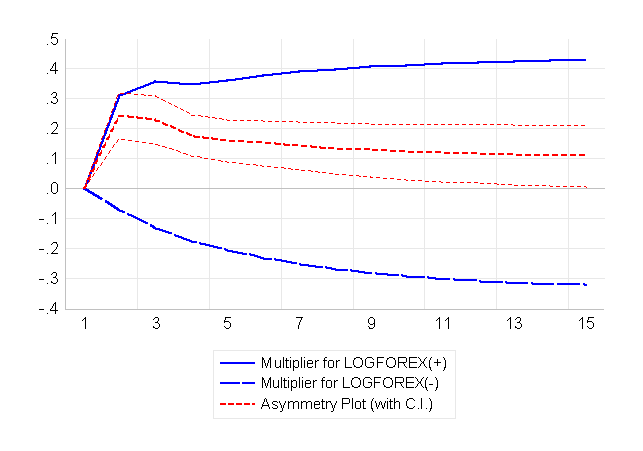
\includegraphics{figures/logequity.png}
    \label{fig:msih_resids}
\end{figure}

De ce graphe, il en sort une implication sur l'asymétrie positive du stress du marché des changes envers le stress sur le marché interbancaire.

\begin{itemize}
    \item \textbf{Multiplicateurs pour $LOGFOREX^+$ (ligne bleue continue) :}
    \begin{itemize}
        \item Les chocs positifs sur LOGFOREX (amélioration des conditions sur le marché des changes) ont un effet initial important et positif sur le stress interbancaire, atteignant un maximum dans les premières périodes (autour de 0,4).
        \item L’effet diminue progressivement mais reste significatif à long terme, indiquant que les effets stabilisateurs des améliorations sur le marché des changes persistent sur plusieurs périodes.
    \end{itemize}

    \item \textbf{Multiplicateurs pour $LOGFOREX^-$ (ligne bleue pointillée) :}
    \begin{itemize}
        \item Les chocs négatifs (détérioration des conditions sur le marché des changes) ont un effet immédiat opposé, plus marqué que les effets positifs dans les premières périodes.
        \item Cet effet décroît plus rapidement à mesure que le temps avance, suggérant que l’impact des chocs négatifs se dissipe plus vite que celui des chocs positifs.
    \end{itemize}

    \item \textbf{Asymétrie (ligne rouge pointillée) :}
    \begin{itemize}
        \item La courbe rouge illustre la différence entre les multiplicateurs positifs et négatifs.
        \item L’asymétrie est clairement visible, avec un effet initialement plus important des chocs positifs sur le marché des changes. Cette asymétrie diminue sur le long terme, mais reste significative.
    \end{itemize}
\end{itemize}

Ensuite, il est tracé le graphe des multiplicateurs du marché actions.

\begin{figure}[H]
    \centering
    \caption{Graphique des multiplicateurs pour le LOGEQUITY.}
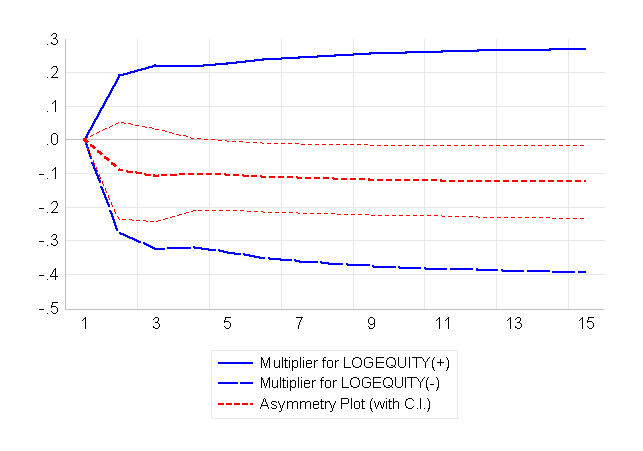
\includegraphics{figures/logforex.png}
    \label{fig:msih_resids}
\end{figure}

De ce graphe, il en sort une implication sur l'asymétrie négative du stress du marché actions envers le stress sur le marché interbancaire.

\begin{itemize}
    \item \textbf{Multiplicateurs pour $LOGEQUITY^+$ (ligne bleue continue) :}
    \begin{itemize}
        \item Les chocs positifs sur LOGEQUITY (hausse du stress sur le marché des actions) ont un effet initial négatif sur le stress interbancaire, ce qui est attendu dans un contexte de tension accrue sur les marchés financiers.
        \item L’effet diminue rapidement après les premières périodes, mais une persistance modérée est observée à long terme.
    \end{itemize}

    \item \textbf{Multiplicateurs pour $LOGEQUITY^-$ (ligne bleue pointillée) :}
    \begin{itemize}
        \item Les chocs négatifs (réduction du stress sur le marché des actions) ont un effet initial beaucoup plus marqué que les chocs positifs.
        \item L’effet reste dominant sur le long terme, indiquant que la détente sur le marché des actions favorise durablement une réduction du stress interbancaire.
    \end{itemize}

    \item \textbf{Asymétrie (ligne rouge pointillée) :}
    \begin{itemize}
        \item Une forte asymétrie est observée, les effets des chocs négatifs étant nettement plus importants que ceux des chocs positifs, tant à court terme qu’à long terme.
        \item Cette asymétrie reflète l'importance des périodes de calme sur les marchés actions pour la stabilité du marché interbancaire.
    \end{itemize}
\end{itemize}

Globalement, 

\begin{itemize}
    \item Les graphiques montrent des dynamiques asymétriques entre les effets positifs et négatifs des variables explicatives. Ces asymétries sont particulièrement marquées pour LOGEQUITY, où les périodes de détente (chocs négatifs) ont un effet stabilisateur bien plus important que les périodes de tension (chocs positifs).
    \item Pour LOGFOREX, l’asymétrie est moins prononcée, mais les chocs positifs jouent un rôle stabilisateur plus durable que les chocs négatifs.
    \item Ces résultats mettent en évidence l'importance d’une gestion proactive des tensions sur les marchés financiers, en ciblant les périodes de volatilité négative (\(LOGFOREX^-\)) et en capitalisant sur les périodes de calme relatif (\(LOGEQUITY^-\)).
\end{itemize}

L'analyse des multiplicateurs dynamiques a mis en évidence des asymétries significatives et une persistance des effets sur le stress interbancaire. Ces résultats soulignent l'importance de comprendre les dynamiques de transmission des chocs entre les marchés financiers et la manière dont ils influencent la stabilité globale du système.\\

Cependant, pour garantir la robustesse des relations modélisées, il faut évaluer la stabilité structurelle du modèle NARDL sur l’ensemble de la période étudiée. À cette fin, le test CUSUM permet d'examiner si les coefficients estimés restent constants dans le temps ou si des changements structurels se manifestent, notamment à la suite de chocs récents.

\begin{figure}[H]
    \centering
    \caption{Test de CUSUM sur le modèle NARDL du LOGIMM.}
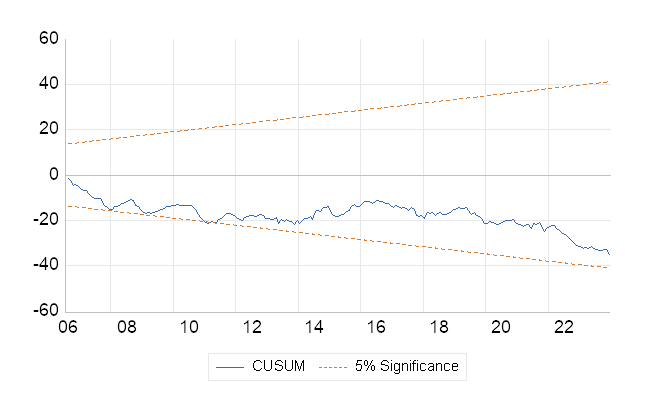
\includegraphics{annexes/cusum_nardl_logequity.png}
    \label{fig:msih_resids}
\end{figure}

La courbe bleue représente le test CUSUM (Cumulative Sum of Recursive Residuals), utilisé pour tester la stabilité des coefficients dans le modèle NARDL. Les lignes en pointillés représentent les bandes de significativité à 5 \%. Si la courbe CUSUM reste à l'intérieur de ces bandes, cela indique que le modèle est structurellement stable sur la période d'estimation.\\

\textbf{Analyse globale de la stabilité :}
\begin{itemize}
    \item La courbe reste bien à l'intérieur des bandes de significativité pendant la quasi-totalité de la période étudiée (2006 à 2022), indiquant une stabilité structurelle des coefficients du modèle.
    \item Une légère tendance à s'éloigner des bandes est observée vers la fin de la période, suggérant des signes potentiels de déviation ou de changement structurel dans les relations modélisées à partir de 2021–2022.
    \item Cela pourrait refléter des perturbations récentes, comme des événements macroéconomiques ou des chocs liés à la pandémie de COVID-19.
\end{itemize}

\textbf{Implications macroprudentielles} \\

\begin{itemize}
    \item Transmission des chocs entre marchés :
    \begin{itemize}
        \item Les asymétries dans les effets de LOGFOREX mettent en évidence un rôle stabilisateur des chocs positifs sur le marché des changes (appréciation des devises). Ces chocs favorisent une réduction modérée du stress interbancaire à court terme (\(M_{CT}^{+} = 0.31\)) et un effet total limité (\(ET^{+} = 0.096494\)). Cet effet stabilisateur persiste néanmoins à long terme (\(\lambda^{LT} = 0.43\)), reflétant une transmission durable de conditions favorables sur le marché des changes vers le marché interbancaire.
        \item À l’inverse, les chocs négatifs (dépréciation des devises) augmentent légèrement le stress interbancaire. L’effet immédiat est faible (\(M_{CT}^{-} = 0.07\)) et l’effet total reste modéré (\(ET^{-} = 0.07\)). Ces résultats suggèrent que le marché interbancaire est relativement résilient aux tensions sur le marché des changes, bien que des dépréciations prolongées puissent entraîner une instabilité accrue, comme le montrent les déviations récentes observées dans le test CUSUM.
        \item Concernant LOGEQUITY, les résultats révèlent une asymétrie marquée. Une hausse du stress sur le marché des actions (\(LOGEQUITY\_POS\)) a un effet immédiat limité (\(M_{CT}^{+} = 0.19\)) et un effet total faible (\(ET^{+} = 0.06\)). En revanche, une baisse du stress (\(LOGEQUITY\_NEG\)) a un impact significativement plus important (\(M_{CT}^{-} = 0.28\) et \(ET^{-} = 0.09\)). Cela reflète un rôle clé des périodes de détente sur le marché des actions pour réduire les tensions interbancaires.
        \item Les graphiques des multiplicateurs confirment ces asymétries et montrent que les chocs positifs (amélioration des conditions) ont des effets persistants mais modérés, tandis que les chocs négatifs (détérioration des conditions) tendent à avoir des effets plus courts mais plus intenses. Ces dynamiques renforcent l'idée que les régulateurs devraient adopter des approches différenciées en fonction de la nature des chocs.
    \end{itemize}

    \item Effets différés et inertie des marchés :
    \begin{itemize}
        \item L’inertie de LOGIMM (\(LOGIMM(-1) = 0.84\)) indique que le stress interbancaire est fortement influencé par ses propres dynamiques passées. Cette persistance peut être attribuée à des mécanismes internes tels que l’ajustement progressif des réserves de liquidité des banques, l’impact des décisions de politique monétaire, ou encore les tensions structurelles sur le marché interbancaire. Cela souligne la nécessité pour les autorités monétaires et régulatrices de surveiller de près l’évolution des tensions afin de limiter une accumulation prolongée de stress.
        \item Les effets différés pour LOGFOREX et LOGEQUITY, notamment les coefficients retardés négatifs (\(-0.22\) et \(-0.19\)), montrent que les ajustements des marchés financiers aux chocs ne sont pas immédiats. Cela implique que les régulateurs disposent d’un délai pour intervenir et mitiger les impacts avant qu’ils ne deviennent systémiques. Toutefois, la persistance observée dans les multiplicateurs à long terme montre également que des chocs prolongés sur les marchés des changes et des actions peuvent entraîner des effets cumulatifs, comme en témoignent les déviations récentes identifiées dans le test CUSUM.
        \item La fin de la période d’estimation (2021–2022) suggère des changements structurels possibles, probablement liés aux chocs externes récents tels que la pandémie de COVID-19, les perturbations géopolitiques (guerre en Ukraine) ou les politiques monétaires restrictives des banques centrales. Ces événements ont pu modifier les relations traditionnelles entre les marchés financiers, nécessitant une réévaluation des modèles et des mécanismes de transmission.
    \end{itemize}

    \item Stabilité structurelle et résilience :
    \begin{itemize}
        \item Le test CUSUM confirme la stabilité structurelle du modèle NARDL sur la majeure partie de la période étudiée (2006–2020), indiquant que les relations entre le stress interbancaire, le marché des changes et le marché des actions restent cohérentes et robustes face aux fluctuations économiques habituelles.
        \item Cependant, les déviations observées vers la fin de la période (2021–2022) signalent des risques potentiels de changements structurels. Ces déviations pourraient refléter une évolution des dynamiques macro-financières sous l’effet des chocs récents. Cela appelle une vigilance accrue de la part des régulateurs pour adapter leurs outils d’analyse et de surveillance aux nouvelles réalités des marchés financiers.
        \item Les résultats mettent en évidence l’importance de mécanismes de coordination entre les banques centrales et les régulateurs pour gérer les interactions entre les différents marchés. Une réponse proactive face aux tensions et une surveillance renforcée des périodes de transition pourraient réduire les risques de contagion systémique.
    \end{itemize}
\end{itemize}

L'estimation du modèle NARDL sur LOGIMM a permis de mettre en évidence des dynamiques asymétriques significatives entre le stress interbancaire et les fluctuations des marchés des changes (LOGFOREX) et des actions (LOGEQUITY). Les résultats montrent que les améliorations sur le marché des changes jouent un rôle stabilisateur durable, tandis que les détériorations sur le marché des actions ont un impact amplifié et persistant sur le stress interbancaire. Ces asymétries, combinées à une inertie marquée du stress interbancaire, soulignent l'importance de comprendre la transmission des chocs entre ces marchés pour renforcer la stabilité financière. Par ailleurs, le test de stabilité structurelle CUSUM confirme la robustesse globale des relations modélisées, bien que des signes de déviation apparaissent en fin de période, reflétant les récents chocs macroéconomiques. Ces résultats mettent en lumière la nécessité d'une surveillance proactive et d'une gestion différenciée des tensions sur les marchés financiers.\\

Après avoir exploré les dynamiques du stress interbancaire, l'analyse se poursuit avec l'estimation d'un modèle NARDL appliqué à LOGEQUITY. Cette démarche vise à comprendre comment les fluctuations asymétriques du stress sur le marché interbancaire (LOGIMM) et sur le marché des changes (LOGFOREX) influencent le stress sur le marché des actions. En particulier, ce modèle permettra d'identifier les asymétries entre les impacts des variations positives et négatives des marchés explicatifs sur le marché des actions. Cela contribuera à évaluer les mécanismes de transmission des chocs financiers, en prenant en compte l'inertie propre au marché des actions et les dynamiques cumulatives associées.

\subsubsection{Estimation d'un modèle NARDL sur le marché actions}

Dans cette seconde application, un modèle NARDL est estimé\footnote{Voir annexe \ref{tab:nardl_logequity} p.\pageref{tab:nardl_logequity}} pour analyser les dynamiques du stress sur le marché des actions, représenté par LOGEQUITY, en réponse aux variations asymétriques du stress sur le marché interbancaire (LOGIMM) et des changes (LOGFOREX). L’objectif est de comprendre comment les fluctuations positives et négatives de ces deux marchés influencent de manière asymétrique le stress sur le marché des actions, tout en intégrant les effets autorégressifs qui traduisent l’inertie propre à ce marché.

\begin{table}[H]
    \centering
    \sffamily
    \caption{Résumé de l'estimation du modèle NARDL sur le LOGEQUITY.}
    \label{tab:estimation_nardl_logequity}
    \begin{tabular}{lcl}
\toprule
\textbf{Variable} & \textbf{Coefficient} & \textbf{Prob.*} \\ % Correction : ajout de "\\" ici
\midrule
$LOGEQUITY_{t-1}$ & $0.46$ & $0.00$ \\
$LOGEQUITY_{t-2}$ & $-0.03$ & $0.00$ \\
$LOGEQUITY_{t-3}$ & $0.18$ & $0.00$ \\
$LOGIMM^+$ & $0.65$ & $0.00$ \\
$LOGIMM^+_{t-1}$ & $-0.47$ & $0.03$ \\
$LOGIMM^-$ & $0.81$ & $0.00$ \\
$LOGIMM^-_{t-1}$ & $-0.62$ & $0.00$ \\
$LOGFOREX^+$ & $0.33$ & $0.00$ \\
$LOGFOREX^+_{t-1}$ & $-0.08$ & $0.03$ \\
$LOGFOREX^+_{t-2}$ & $0.19$ & $0.05$ \\
$LOGFOREX^+_{t-3}$ & $-0.13$ & $0.01$ \\
$LOGFOREX^+_{t-4}$ & $-0.10$ & $0.05$ \\
$LOGFOREX^-$ & $0.21$ & $0.00$ \\
$\phi_0$ & $0.36$ & $0.00$ \\
\midrule % Ligne séparatrice
\textbf{$R^2$} & $0.83$ & \\
Adjusted $R^2$ & $0.82$ & \\
Akaike info criterion & $0.19$ & \\
\midrule % Ligne séparatrice
\textbf{Analyse des résidus} \\ % Analyse des résidus
Homoscedasticité & Corrigé par Newey-West & annexe \ref{tab:arch_nardl_logequity} p.\pageref{tab:arch_nardl_logequity} \\
Autocorrélation & Corrigé par Newey-West & annexe \ref{fig:correlo_nardl_equity} p.\pageref{fig:correlo_nardl_equity} \\
Normalité & JB = 0.69 & normalité des résidus \footnotesize{(\ref{fig:normalite_nardl_logequity}}) \\
\midrule % Ligne séparatrice
\textbf{Tests coefficients NARDL} \\ % Analyse des résidus
Wald-test symétrie & $\chi^2 = 22.05$ & asymétrie valide \footnotesize{(\ref{tab:asymetrie_nardl_logequity} p.\pageref{tab:asymetrie_nardl_logequity})}  \\
Test de redondance & $F_{stat} = 19.49$ & non redondance \footnotesize{(\ref{tab:redondance_nardl_logequity} p.\pageref{tab:redondance_nardl_logequity})}\\
Test RESET Ramsey & $F_{stat} = 0.53$ & pas de polynôme \footnotesize{(\ref{tab:reset_nardl_logequity} p.\pageref{tab:reset_nardl_logequity})} \\
VIF & VIF faibles & pas de colinéarité \footnotesize{(\ref{tab:vif_nardl_logequity} p.\pageref{tab:vif_nardl_logequity})} \\
\bottomrule
\end{tabular}

\end{table}

Après estimation, le modèle peut donc être spécifié comme : 

\begin{align*}
\widehat{LOGEQUITY}_t =\ & 0.36 \\
& + 0.46 \cdot LOGEQUITY_{t-1} - 0.03 \cdot LOGEQUITY_{t-2} + 0.18 \cdot LOGEQUITY_{t-3} \\
& + 0.65 \cdot LOGIMM^{+}_t - 0.47 \cdot LOGIMM^{+}_{t-1} \\
& + 0.81 \cdot LOGIMM^{-}_t - 0.62 \cdot LOGIMM^{-}_{t-1} \\
& + 0.33 \cdot LOGFOREX^{+}_t - 0.08 \cdot LOGFOREX^{+}_{t-1} + 0.19 \cdot LOGFOREX^{+}_{t-2} \\
& - 0.13 \cdot LOGFOREX^{+}_{t-3} - 0.10 \cdot LOGFOREX^{+}_{t-4} \\
& + 0.21 \cdot LOGFOREX^{-}_t 
\end{align*}

Les coefficients obtenus ainsi que les multiplicateurs calculés mettent en évidence plusieurs points clés :

\begin{itemize}
    \item \textbf{Structure autorégressive de LOGEQUITY :}
    \begin{itemize}
        \item Le coefficient de \(LOGEQUITY_{t-1} = 0.463576\) montre une inertie modérée du stress sur le marché des actions. Cela suggère que les dynamiques passées influencent significativement le stress actuel, mais moins fortement que dans le modèle LOGIMM.
        \item Les coefficients retardés \(LOGEQUITY_{t-2}\) et \(LOGEQUITY_{t-3}\) indiquent des ajustements mineurs à moyen terme, ce qui est cohérent avec un rééquilibrage progressif des flux financiers après des chocs initiaux.
    \end{itemize}

    \item \textbf{Asymétrie dans les effets de LOGIMM :}
    \begin{itemize}
        \item Les chocs positifs (\(LOGIMM^{+} = 0.65\)) augmentent significativement le stress sur le marché des actions. Cet effet est partiellement compensé par un ajustement retardé négatif (\(LOGIMM^{+}_{t-1} = -0.47\)), ce qui peut refléter une réallocation de liquidité entre les marchés.
        \item Les chocs négatifs (\(LOGIMM^{-} = 0.81\)) ont un effet encore plus marqué, augmentant considérablement le stress sur LOGEQUITY. Cela illustre une transmission amplifiée des tensions interbancaires vers le marché des actions en période de crise.
    \end{itemize}

    \item \textbf{Asymétrie dans les effets de LOGFOREX :}
    \begin{itemize}
        \item Les variations positives (\(LOGFOREX^{+} = 0.33\)) ont un effet immédiat significatif, réduisant le stress sur LOGEQUITY. Cependant, cet effet est atténué à moyen terme par des coefficients retardés négatifs (\(-0.1\)).
        \item Les variations négatives (\(LOGFOREX^{-} = 0.21\)) augmentent modérément le stress sur LOGEQUITY, mais de manière moins marquée que les effets des variations positives.
    \end{itemize}
\end{itemize}

Ces résultats préliminaires mettent en évidence des dynamiques asymétriques significatives dans la transmission des chocs interbancaires et des changes vers le stress sur le marché des actions. L'inertie modérée de LOGEQUITY reflète une dépendance importante aux dynamiques passées, tandis que les effets des variations positives et négatives de LOGIMM et LOGFOREX soulignent des asymétries marquées, notamment en période de crise.Les chocs positifs sur le marché interbancaire semblent induire un rééquilibrage financier qui limite leur impact à moyen terme, tandis que les tensions interbancaires négatives amplifient fortement le stress sur les actions. De même, les améliorations sur le marché des changes jouent un rôle stabilisateur sur le stress actions, bien que leur effet s’atténue sur le long terme.\\

Pour compléter cette analyse et mieux comprendre l'ampleur et la persistance des impacts, l'étude des multiplicateurs dynamiques est essentielle. Ces multiplicateurs permettent d’évaluer l’intensité des effets à court, moyen et long terme, et de confirmer les asymétries observées dans les coefficients estimés. Passons désormais à cette analyse approfondie des multiplicateurs.

\vspace{0.5cm}

\textbf{Analyse des multiplicateurs} \\

Les multiplicateurs calculés pour ce modèle NARDL, une fois calculés, sont résumés dans le tableau ci-après.

\begin{table}[H]
\centering
\sffamily
\caption{Multiplicateurs et effets totaux pour LOGIMM et LOGFOREX sur LOGEQUITY.}
\label{tab:multiplicateurs_logequity}
\begin{tabular}{llccc}
\toprule
\textbf{Variable}   & \textbf{Type}          & \textbf{(\(M_{CT}\))} & \textbf{(\(ET\))} & \textbf{(\(\lambda^{LT}\))} \\ \midrule
{LOGIMM} & Positif (\(+\))    & \( 0.65 \)           & \( 0.47 \)           & \( 0.50 \)        \\ 
         & Négatif (\(-\))    & \( 0.81 \)           & \( 0.90 \)           & \( 0.72 \)        \\ \midrule
{LOGFOREX} & Positif (\(+\))   & \( 0.33 \)           & \( 0.27 \)           & \( 0.38 \)        \\  
           & Négatif (\(-\))   & \( 0.21 \)           & \( 0.12 \)           & \( 0.18 \)        \\ \bottomrule
\end{tabular}
\end{table}

Les multiplicateurs associés à LOGIMM et LOGFOREX permettent de comprendre comment les variations positives et négatives de ces variables influencent le stress sur le marché des actions (LOGEQUITY) à court terme, en effet total et sur le long terme.\\

Impacts asymétriques du marché interbancaire :\\

\begin{itemize}
    \item \textbf{Court terme (\(M_{CT}\)) :} 
    Les chocs positifs sur le marché interbancaire (\(M_{CT}^+ = 0.65\)) ont un effet immédiat significatif sur le stress des actions. Cela reflète une transmission rapide des améliorations interbancaires vers le marché des actions, qui peut être due à une amélioration de la liquidité globale ou à une réduction des incertitudes sur les marchés financiers.  
    À l’inverse, les chocs négatifs (\(M_{CT}^- = 0.81\)) exercent un effet immédiat plus marqué, traduisant une sensibilité accrue du marché des actions aux tensions interbancaires. Cela souligne un phénomène de contagion, où les perturbations sur le marché interbancaire se propagent rapidement et amplifient le stress sur le marché des actions.

    \item \textbf{Effet total (\(ET\)) :} 
    L’effet cumulé des chocs négatifs (\(ET^- = 0.90\)) dépasse largement celui des chocs positifs (\(ET^+ = 0.47\)). Cela indique que les tensions interbancaires ont un impact prolongé et amplifié sur le stress actions, tandis que les améliorations interbancaires ont un effet atténué. Cette asymétrie souligne la vulnérabilité des marchés financiers en période de crise interbancaire.

    \item \textbf{Long terme (\(\lambda^{LT}\)) :} 
    Les multiplicateurs de long terme confirment cette asymétrie : les effets négatifs (\(\lambda^{LT}_{LOGIMM^-} = 0.72\)) persistent davantage que les effets positifs (\(\lambda^{LT}_{LOGIMM^+} = 0.50\)). Cela illustre que les tensions interbancaires prolongées peuvent entraîner une instabilité durable sur le marché des actions, nécessitant des interventions régulatrices ciblées pour atténuer les risques systémiques.
\end{itemize}

Impacts asymétriques du marché des changes :\\

\begin{itemize}
    \item \textbf{Court terme (\(M_{CT}\)) :} 
    Les variations positives sur le marché des changes (\(M_{CT}^+ = 0.33\)) exercent un effet immédiat stabilisateur sur le stress actions, reflétant l’impact positif des améliorations sur le marché des devises sur la confiance des investisseurs et la stabilité financière.  
    En revanche, les chocs négatifs (\(M_{CT}^- = 0.21\)) ont un effet moins marqué à court terme, suggérant une certaine résilience du marché des actions face aux tensions modérées sur le marché des changes.

    \item \textbf{Effet total (\(ET\)) :} 
    L’effet cumulé des variations positives (\(ET^+ = 0.27\)) est supérieur à celui des variations négatives (\(ET^- = 0.12\)). Cela confirme le rôle stabilisateur des améliorations sur le marché des changes, bien que leur impact global soit modéré par rapport à LOGIMM.

    \item \textbf{Long terme (\(\lambda^{LT}\)) :} 
    Les multiplicateurs de long terme montrent une asymétrie plus marquée : les variations positives (\(\lambda^{LT}_{LOGFOREX^+} = 0.38\)) ont un effet plus persistant que les variations négatives (\(\lambda^{LT}_{LOGFOREX^-} = 0.18\)). Cela reflète l’importance d’un marché des changes stable pour atténuer les tensions sur le marché des actions sur une période prolongée.
\end{itemize}

Les tensions interbancaires amplifient fortement le stress actions, avec un impact plus important et persistant des chocs négatifs. Cela illustre un mécanisme de contagion où les crises interbancaires se propagent systématiquement vers les autres segments financiers. Les améliorations sur le marché des changes jouent un rôle stabilisateur, réduisant durablement les tensions sur le marché des actions, tandis que les chocs négatifs ont un impact plus modéré.\\

Ces dynamiques asymétriques renforcent l'importance d'une surveillance proactive des tensions sur les marchés interbancaire et des changes pour limiter leur impact systémique sur le marché des actions. Il convient désormais d'étudier le stabilité.

\vspace{0.5cm}

\textbf{Analyse des multiplicateurs et test CUSUM} \\

Les graphiques montrent l’évolution des multiplicateurs dynamiques des variations positives et négatives pour LOGIMM et LOGFOREX sur LOGEQUITY à travers plusieurs périodes (horizons temporels). Ces graphiques aident à comprendre les asymétries et la persistance des effets sur le stress du marché des actions. Il est d'abord tracé le graphe des multiplicateurs pour le stress sur le marché interbancaire.

\begin{figure}[H]
    \centering
    \caption{Graphique des multiplicateurs pour LOGIMM.}
    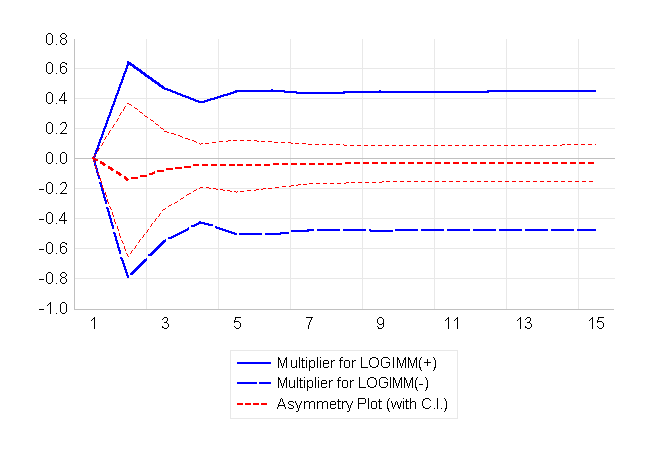
\includegraphics{figures/multiplier_logimm.png}
    \label{fig:multiplier_logimm}
\end{figure}

Il en sort une asymétrie négative et des effets de court terme divergents détaillés ci-après.

\begin{itemize}
    \item \textbf{Multiplicateurs pour $LOGIMM^+$ (ligne bleue continue) :}
    \begin{itemize}
        \item Les chocs positifs sur LOGIMM augmentent immédiatement le stress sur LOGEQUITY, atteignant un pic significatif dans les premières périodes (\(\approx 0.6\)).
        \item Cet effet diminue progressivement mais reste significatif à moyen terme.
    \end{itemize}

    \item \textbf{Multiplicateurs pour $LOGIMM^-$ (ligne bleue pointillée) :}
    \begin{itemize}
        \item Les chocs négatifs sur LOGIMM ont un effet encore plus marqué sur le stress des actions, atteignant un pic initial plus élevé (\(\approx 0.8\)).
        \item Cet effet décroît plus lentement, montrant une persistance importante des tensions interbancaires négatives sur le marché des actions.
    \end{itemize}

    \item \textbf{Asymétrie (ligne rouge pointillée) :}
    \begin{itemize}
        \item Une asymétrie claire est observée, les chocs négatifs ayant un effet plus important et persistant que les chocs positifs.
        \item Cette asymétrie reflète une amplification des tensions interbancaires en période de crise.
    \end{itemize}
\end{itemize}

Ensuite, est tracé le graphe des multiplicateurs pour le stress du marché des changes et son impact sur le stress du marché actions.

\begin{figure}[H]
    \centering
    \caption{Graphique des multiplicateurs pour LOGFOREX.}
    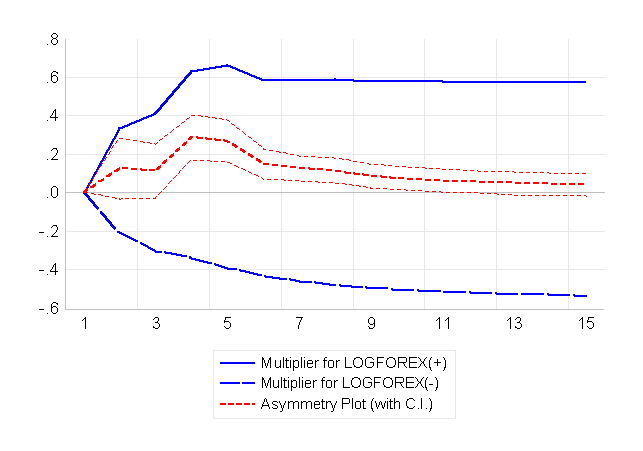
\includegraphics{figures/multiplier_logforex.png}
    \label{fig:multiplier_logforex}
\end{figure}

Il en sort une asymétrie par pallier positive qui met en évidence des mouvements de correctioon et d'assimilation sur les marchés actions.

\begin{itemize}
    \item \textbf{Multiplicateurs pour $LOGFOREX^+$ (ligne bleue continue) :}
    \begin{itemize}
        \item Les chocs positifs sur LOGFOREX (amélioration des conditions sur le marché des changes) réduisent immédiatement le stress sur LOGEQUITY (\(\approx 0.33\)).
        \item Cet effet diminue progressivement mais reste significatif à moyen terme.
    \end{itemize}

    \item \textbf{Multiplicateurs pour $LOGFOREX^-$ (ligne bleue pointillée) :}
    \begin{itemize}
        \item Les chocs négatifs sur LOGFOREX augmentent modérément le stress sur LOGEQUITY (\(\approx 0.21\)).
        \item Ces effets sont moins persistants par rapport aux chocs positifs.
    \end{itemize}

    \item \textbf{Asymétrie (ligne rouge pointillée) :}
    \begin{itemize}
        \item Une asymétrie est observée, les chocs positifs ayant un effet plus stabilisateur que les chocs négatifs.
        \item Cela reflète un rôle stabilisateur durable du marché des changes sur les tensions du marché des actions.
    \end{itemize}
\end{itemize}

\vspace{0.5cm}

Enfin, le test CUSUM est effectué pour juger de la stabilité des paramètres du modèle.

\begin{figure}[H]
    \centering
    \caption{Test de CUSUM sur le modèle NARDL du LOGEQUITY.}
    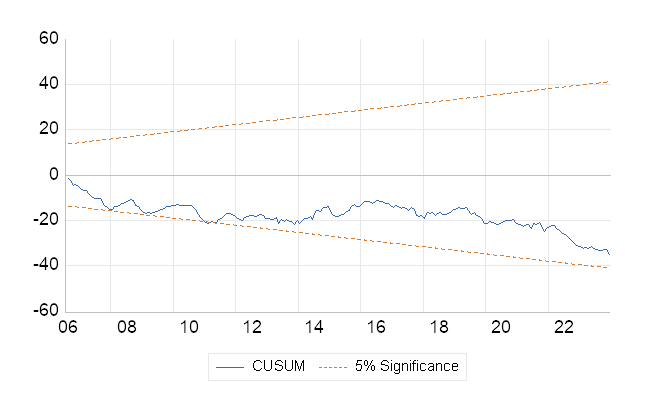
\includegraphics{annexes/cusum_nardl_logequity.png}
    \label{fig:cusum_logequity}
\end{figure}

Comme précédemment, la courbe bleue représente le test CUSUM (Cumulative Sum of Recursive Residuals), utilisé pour tester la stabilité des coefficients dans le modèle NARDL. Les lignes en pointillés représentent les bandes de significativité à 5 \%. Si la courbe CUSUM reste à l'intérieur de ces bandes, cela indique que le modèle est structurellement stable.\\

\textbf{Analyse de la stabilité :}
\begin{itemize}
    \item La courbe reste bien à l'intérieur des bandes de significativité pendant presque toute la période étudiée (2006 à 2022), indiquant une stabilité structurelle.
    \item Une légère déviation vers la fin de la période (2021–2022) pourrait refléter des changements structurels potentiels, liés à des événements récents tels que la pandémie de COVID-19 ou des tensions géopolitiques.
\end{itemize}

\vspace{0.5cm}

\textbf{Implications macroprudentielles} \\

\begin{itemize}
    \item \textbf{Transmission des chocs entre marchés :}
    \begin{itemize}
        \item Les graphiques des multiplicateurs pour LOGIMM et LOGFOREX montrent des asymétries marquées dans la transmission des chocs vers \(LOGEQUITY\), le stress sur le marché des actions. Ces asymétries mettent en évidence la forte interconnexion entre ces trois segments des marchés financiers.
        \item Les chocs négatifs sur LOGIMM (\(LOGIMM\_NEG\)), représentant des tensions accrues sur le marché interbancaire, amplifient fortement le stress sur les actions, avec des effets immédiats importants (\(M_{CT}^{-} = 0.81\)) et persistants (\(\lambda^{LT}_{LOGIMM\_NEG} = 0.72\)). Cette transmission indique qu’en période de crise interbancaire, la dégradation de la liquidité interbancaire et la méfiance entre institutions financières se répercutent rapidement sur les marchés actions.
        \item Les chocs positifs sur LOGIMM (\(LOGIMM\_POS\)) augmentent temporairement le stress sur le marché des actions (\(M_{CT}^{+} = 0.65\)), mais cet effet diminue à moyen terme grâce à une réallocation des flux financiers vers des actifs plus risqués, reflétant un regain de confiance des investisseurs.
        \item Concernant LOGFOREX, les chocs positifs (\(LOGFOREX\_POS\)), qui reflètent une amélioration des conditions sur le marché des changes, jouent un rôle stabilisateur significatif sur LOGEQUITY (\(M_{CT}^{+} = 0.33\), \(\lambda^{LT}_{LOGFOREX\_POS} = 0.38\)). Cette relation met en évidence l'importance d'un marché des changes stable pour soutenir la confiance sur les marchés actions.
        \item Les chocs négatifs sur LOGFOREX (\(LOGFOREX\_NEG\)), bien qu’ils augmentent le stress sur les actions (\(M_{CT}^{-} = 0.21\)), ont des effets moins marqués et moins persistants (\(\lambda^{LT}_{LOGFOREX\_NEG} = 0.18\)), reflétant une résilience relative des actions face aux tensions modérées sur le marché des changes.
    \end{itemize}

    \item \textbf{Stabilité structurelle et signaux de vulnérabilité :}
    \begin{itemize}
        \item Le test CUSUM indique que le modèle est structurellement stable pour la période 2006–2022, ce qui signifie que les relations entre le stress sur les marchés actions, interbancaire et des changes sont restées constantes sous des conditions de marché normales.
        \item Cependant, des déviations observées en fin de période (2021–2022) suggèrent de possibles changements structurels, possiblement dus à des perturbations exogènes majeures comme la pandémie de COVID-19 ou des tensions géopolitiques. Ces événements auraient pu modifier les comportements des acteurs de marché, en exacerbant les interconnexions entre ces trois segments financiers.
        \item Ces signaux de vulnérabilité exigent une vigilance accrue des autorités régulatrices, particulièrement en périodes de transition ou de volatilité élevée.
    \end{itemize}

    \item \textbf{Rôle des politiques monétaires et de change :}
    \begin{itemize}
        \item Les résultats soulignent que les améliorations sur le marché des changes (\(LOGFOREX\_POS\)) réduisent efficacement les tensions sur les marchés actions, reflétant l’importance d’un marché des changes stable pour absorber les chocs exogènes. Les banques centrales devraient donc intégrer des interventions ciblées sur ce marché pour renforcer la confiance des investisseurs.
        \item À l’inverse, les crises interbancaires (\(LOGIMM\_NEG\)) exacerbent significativement le stress sur les actions. Cela indique que les régulateurs devraient prioriser des mécanismes de stabilisation interbancaire, comme des garanties de liquidité, pour limiter les effets de contagion vers les autres segments financiers.
    \end{itemize}

    \item \textbf{Gestion des risques et stratégies de résilience :}
    \begin{itemize}
        \item Les asymétries mises en évidence montrent que les périodes de crise nécessitent des interventions plus importantes et spécifiques. En particulier, les chocs interbancaires négatifs ont des effets prolongés et intenses, nécessitant des mécanismes de gestion des crises robustes, comme une augmentation des réserves obligatoires ou des injections de liquidités par les banques centrales.
        \item Les ajustements retardés observés dans les effets de LOGIMM et LOGFOREX indiquent que les marchés ne réagissent pas instantanément aux chocs. Cette inertie offre une opportunité pour des interventions régulatrices avant que les tensions ne se propagent de manière systémique.
        \item Une coordination internationale est essentielle, notamment pour les tensions sur le marché des changes, qui peuvent avoir des répercussions transfrontalières sur les actions. Des cadres macroprudentiels globaux peuvent aider à prévenir les risques de contagion.
    \end{itemize}

    \item \textbf{Implications pour la surveillance macroprudentielle :}
    \begin{itemize}
        \item La forte interconnexion entre les marchés des actions, interbancaire et des changes suggère que les régulateurs devraient adopter une surveillance intégrée, en mettant l'accent sur les indicateurs avancés tels que les multiplicateurs dynamiques.
        \item Les asymétries observées entre les chocs positifs et négatifs montrent que les outils de régulation doivent être différenciés. Par exemple, des interventions proactives pourraient être déployées lors des chocs interbancaires négatifs, tandis que les périodes de calme sur le marché des changes devraient être utilisées pour renforcer les marges de sécurité.
    \end{itemize}
\end{itemize}

Les résultats de ce projet apportent des éclairages essentiels sur les interactions dynamiques entre les sous-indicateurs de stress systémique, à savoir le marché des changes (LOGFOREX), le marché interbancaire (LOGIMM), et le marché des actions (LOGEQUITY). Les modèles MS-VAR ont révélé des effets significatifs de transmission entre ces segments, soulignant l’importance des interconnexions dans la propagation du stress financier. Par exemple, un choc sur le marché interbancaire se traduit par une amplification du stress sur le marché des changes dans un laps de temps court, tandis que l’impact sur le marché des actions est plus diffus, bien que durable.\\

L’analyse a également permis de mettre en évidence des asymétries importantes. En particulier, les phases de stress élevé (régimes "haut") exacerbent la transmission des chocs entre les marchés, alors que dans les périodes de faible stress (régimes "bas"), les interactions sont moins marquées. Cette asymétrie est cruciale pour les régulateurs, car elle indique que les mécanismes de transmission varient selon les conditions de marché.\\

Un autre résultat est la contribution différenciée de chaque sous-indicateur au stress global. Le marché interbancaire joue un rôle central en tant que vecteur initial de propagation, confirmant son statut de baromètre de la stabilité financière. En revanche, le marché des changes semble réagir davantage comme un amplificateur, particulièrement vulnérable aux perturbations provenant des autres segments. Ces dynamiques différenciées appellent à une surveillance accrue du marché interbancaire, tout en intégrant des mécanismes de réaction rapide pour limiter les effets d’amplification sur les marchés périphériques (justement comme le FOREX).\\

Pour les régulateurs, ces résultats soulignent la nécessité d’approches différenciées en fonction des segments de marché et des régimes de stress. Une régulation macroprudentielle proactive, combinée à des indicateurs avancés basés sur des modèles multivariés, pourrait permettre de mieux anticiper les épisodes de contagion systémique. De plus, l’intégration d’indicateurs asymétriques dans les cadres de surveillance pourrait améliorer la réactivité des politiques en fonction des conditions de marché.\\
